\ifnum\aluno=1
\renewcommand\chapterillustration{./abertura-trigonometrica}
\else
\renewcommand\chapterillustration{./abertura-trigonometrica-professor}
\fi


\def\chapterwhat{Fenômenos Periódicos, Radiano, Funções Seno e Cosseno, Senóides.}
\def\chapterbecause{Fenômenos periódicos são aqueles que se repetem com o tempo. Alguns exemplos de tais fenômenos são os batimentos cardíacos, as fases da lua, do nascer do sol, o movimento dos ponteiros de um relógio ou de um pêndulo. O próprio movimento de rotação da Terra é um fenômeno periódico que se repete em períodos de 24 horas, sendo o responsável pelas noções de dia e de noite. As funções trigonométricas, diferente das demais que estudamos até aqui, têm a propriedade de serem periódicas, isto é, seus gráficos se replicam ciclicamente em intervalos determinados do seu domínio. Esta característica faz dessas funções as mais adequadas para modelar matematicamente e prever informações sobre os fenômenos periódicos.} 
\chapter{Funções Trigonométricas}
\label{trigo-chap}

\mbox{}\thispagestyle{empty}\clearpage

\thispagestyle{empty}

\begin{center}
Projeto: LIVRO ABERTO DE MATEMÁTICA

\noindent \begin{tabular}{lcccr}

\includegraphics[scale=.15]{impa}& \quad\quad& 
\includegraphics[width=3cm]{logo} & \quad\quad& 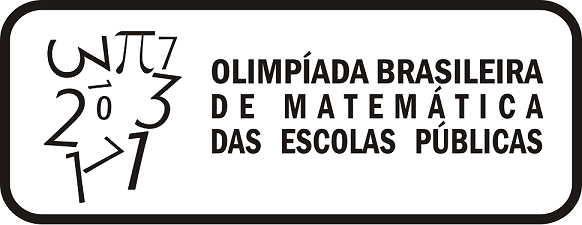
\includegraphics[scale=.24]{obmep} 
\end{tabular}
\end{center}

\vspace*{.3cm}

Cadastre-se como colaborador no site do projeto: \url{umlivroaberto.org}



% \begin{center}
%   \includegraphics[width=2cm]{canvas}
% \end{center}

\begin{tabular}{p{.15\textwidth}p{.7\textwidth}}
Título: & Funções Trigonométricas\\
\\
Ano/ Versão: & 2020 / versão 0.2 de 17 de novembro de 2020\\
\\
Editora & Instituto Nacional de Matem\'atica Pura e Aplicada (IMPA-OS)\\
\\
Realização:& Olimp\'iada Brasileira de Matem\'atica das Escolas P\'ublicas (OBMEP)\\
\\
Produção:& Associação Livro Aberto\\
\\
Coordenação: & Fabio Simas, \\
			&  Augusto Teixeira (livroaberto@impa.br)\\
\\
  Autor: & Ivail Muniz Junior\\
        
\\
Colaboração: & \\
\\
Revisor: & Amarildo Melchiades da Silva \\
         & Vanessa Matos \\
\\
Design: & Andreza Moreira (Tangentes Design) \\
\\
  Ilustrações: & --- \\ 
\\
Gráficos: & Tarso Caldas (Licenciando da UNIRIO)\\
\\
  Capa: & Foto de Josh Appel, no Unsplash \\
  		& https://unsplash.com/photos/QSipy5RFcSA \\

\end{tabular}
\vspace{.5cm}



\begin{figure}[b]
\begin{minipage}[l]{5cm}
\centering

{\large Licença:}

  
\includegraphics[width=3.5cm]{cc-by-nc-sa}
\end{minipage}\hfill
\begin{minipage}[c]{5cm}
\centering
{\large Desenvolvido por}


\includegraphics[width=2.5cm]{logo-associacao.jpg}
\end{minipage}
\begin{minipage}[r]{5cm}
\centering

{\large Patrocínio:}
  \vspace{1em}
  
\includegraphics[width=3.5cm]{itau}
\end{minipage}
\end{figure}

\mainmatter


\explore{Fenômenos Periódicos}
\label{trig-exp1}

Iniciaremos este capítulo estudando exemplos de fenômenos do nosso cotidiano que têm uma propriedade até então não observada nos capítulos anteriores do livro de Funções: são fenômenos que se repetem com o passar do tempo. Um dos objetivos desse capítulo é estudar técnicas de modelagem matemática desse tipo de fenômeno, visando antever situações relacionadas a ele. Quais seriam as funções adequadas para realizar essa modelagem? Realizando as atividades a seguir, você irá aos poucos descobrir que funções são essas e que características algébricas e gráficas elas possuem.



\begin{task}{Pêndulo de um relógio}
\textit{(Adaptado de \cite{costa2017})}
\label{trig-ativ1}

Alguns relógios rústicos têm um pêndulo, composto por uma bolinha presa à parte de baixo de uma haste que oscila continuamente de um lado para o outro. O fato de o pêndulo estar em movimento mostra que o relógio está em pleno funcionamento.

\begin{figure}[H]
\centering

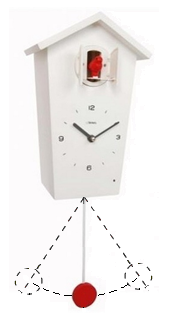
\includegraphics[width=.25\linewidth]{trigonometricas1}
\end{figure}

Vamos estudar o comportamento da projeção do centro dessa bola numa reta horizontal localizada abaixo desse relógio, supondo que a origem dessa reta coincida com a projeção do centro da bola quando a haste do pêndulo está na posição vertical. Em outras palavras, vamos estudar as variações dos pontos da reta alcançados pela projeção do centro da bola. As imagens a seguir ilustram algumas possíveis posições do pêndulo. O centro do pêndulo está representado pelo ponto $E$; os pontos $C$ e $B$ são os pontos extremos do caminho percorrido pelo pêndulo. O ponto $O$ é aquele em que o pêndulo se encontra preso ao relógio. O ponto $F$ indica possíveis posições do pêndulo, e o ponto $G$ indica a projeção de $E$ na reta orientada a seguir. Observe as diferentes posições de $F$ ilustradas e os valores da distância entre $A$ e $G$ ($A$ é a projeção de $O$ na reta orientada). A construção no GeoGebra do movimento de um pêndulo similar a esse pode ser acessada no link \url{https://www.geogebra.org/classic/uxcqamaz}


\begin{figure}[H]
\centering

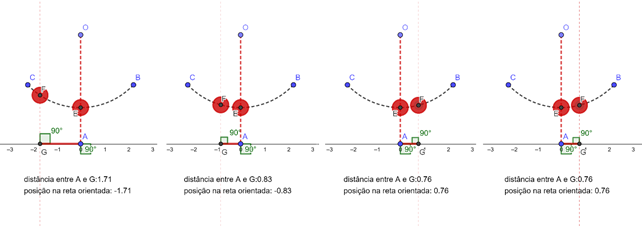
\includegraphics[width=\linewidth]{trigonometricas2}
\end{figure}

Suponha que no tempo $t$, a função que descreve o deslocamento dessa projeção seja $d(t)$. Note que, como estabelecemos uma posição como origem, esta função é considerada com sinal assumindo um valor positivo quando o pêndulo estiver à direita do segmento $OA(d(t_1)\geq0)e$ assumindo um valor negativo quando estiver à esquerda de $OA(d(t_2)\leq0)$, conforme é possível ver na ilustração acima: a distância entre $A$ e $G$ é um módulo, é absoluta; no entanto, quando consideramos a posição na reta orientada, atribuímos um sinal a essa distância.

\begin{figure}[H]
\centering

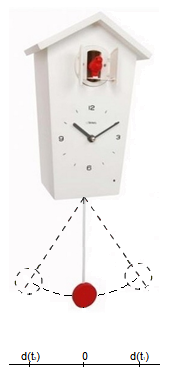
\includegraphics[width=.25\linewidth]{trigonometricas3}
\end{figure}

\begin{enumerate}
\item Na malha quadriculada abaixo, considere $D\max$ e $E\max$ o maior e o menor valor assumidos pela função $d$. Repare que $D\max$ corresponde à projeção do ponto $B$ na reta horizontal, que é o ponto mais à direita que é atingido pelo centro da bolinha ao longo da oscilação do pêndulo. Da mesma forma, $E\max$ corresponde à projeção de $C$, que é o ponto mais à esquerda que é atingido pelo centro da bolinha durante o movimento. Tente esboçar o gráfico da função $d(t)$, supondo que d(0) = $D\max$.

\begin{figure}[H]
\centering

\resizebox{.75\linewidth}{!}
{
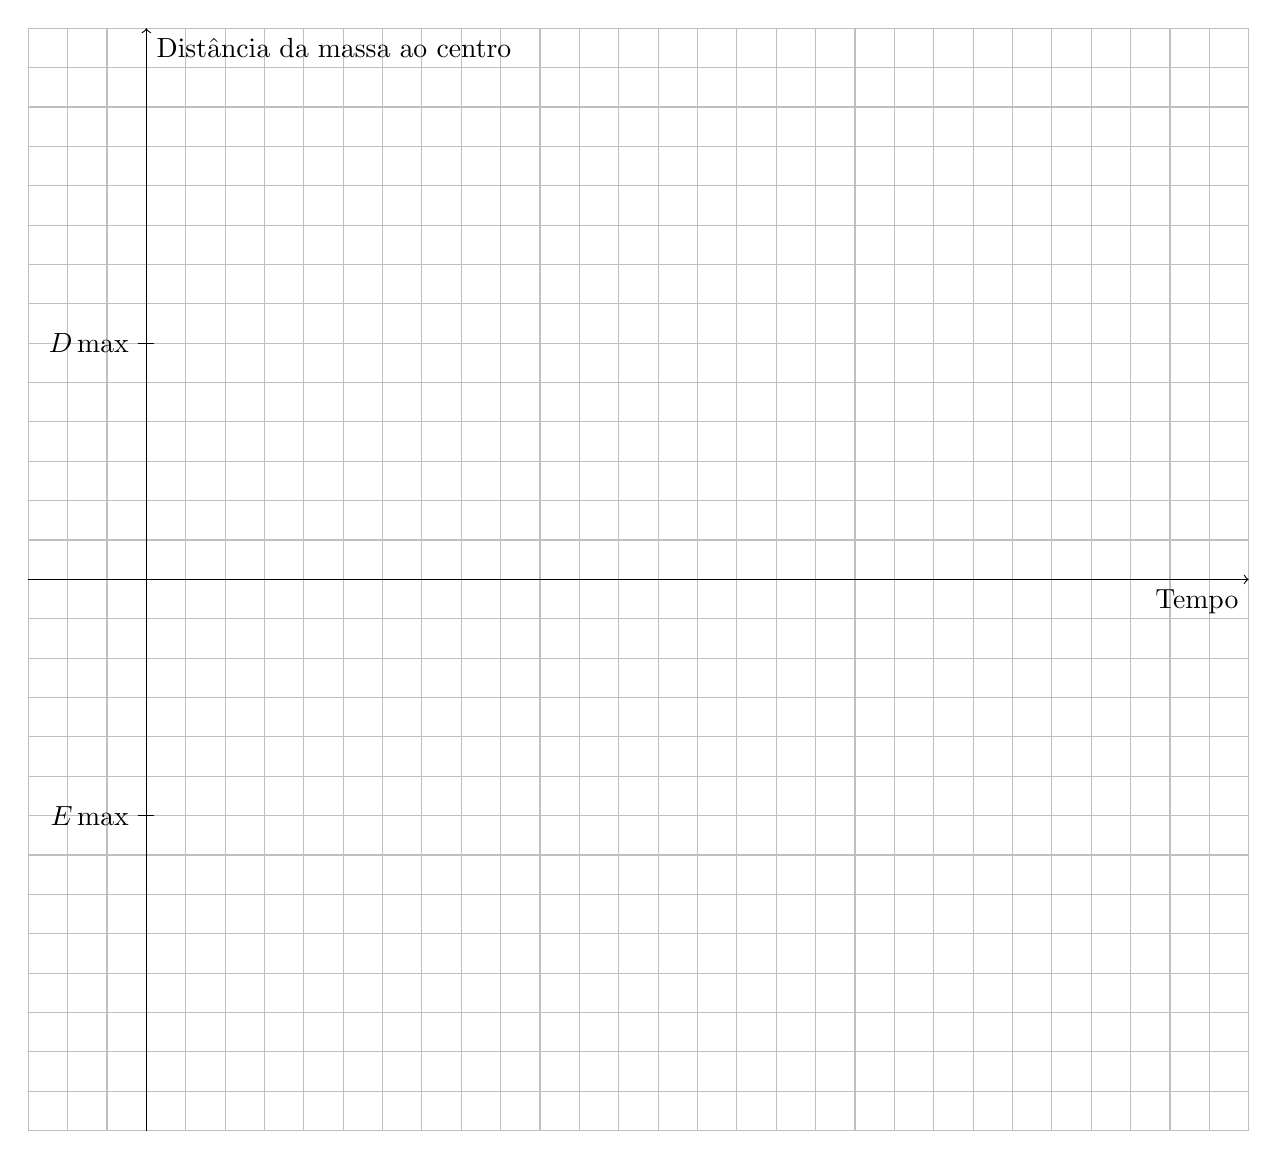
\begin{tikzpicture}
\draw [step=.5,gray!50] (-1.5,-7) grid (14,7);
\draw [->] (-1.5,0) -- (14,0) node [below left, thick] {Tempo};
\draw [->] (0,-7) -- (0,7) node [below right, thick] {Distância da massa ao centro};
\draw (.1,3) -- (-.1,3) node [left, overlay] {$D\max$};
\draw (.1,-3) -- (-.1,-3) node [left, overlay] {$E\max$};
\end{tikzpicture}
}
\end{figure}

\item Que aspectos você percebe que esse gráfico possui? Cite algumas diferenças entre ele e os gráficos das funções que você estudou até aqui.
\end{enumerate}
\end{task}

\begin{task}{Construindo o próprio pêndulo}
\textit{(Adaptado de \cite{costa2017})}
\label{trig-ativ2}

Com madeira, um prego, barbante e uma bolinha de gude, construir um pêndulo como o da figura. 

\begin{figure}[H]
\centering

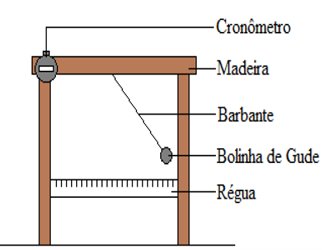
\includegraphics[height=.225\textheight]{trigonometricas5}
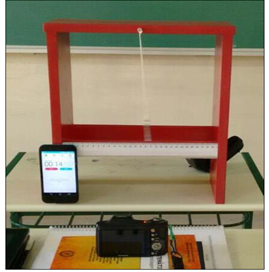
\includegraphics[height=.225\textheight]{trigonometricas6}

\caption{\cite{costa2017}}
\end{figure}

Será necessário o uso de dois celulares ou um celular e uma câmera. Um dos celulares irá cronometrar o tempo durante a oscilação do pêndulo e o outro, deverá tirar sucessivas fotografias do movimento do pêndulo e do primeiro celular. Uma régua deve ser utilizada também para medir o deslocamento horizontal da projeção do pêndulo, como na figura acima. Posicione o pêndulo exatamente sobre o zero da régua e solte-o no momento em que cronômetro for ligado e as fotos começarem a ser tiradas. Fotografar o movimento ao longo de 4 oscilações completas do pêndulo.

\begin{enumerate}
\item Analise as fotografias e forme pares ordenados $(x,y)$ onde $x$ representa o tempo e $y$, a medida na régua na qual estará a projeção horizontal do pêndulo.

\item Plote os pontos no GeoGebra. Que comportamento você consegue perceber no caminho que os pontos vão percorrendo?
\item Compare o esboço que você obteve aqui com o da atividade anterior. Que conclusões você consegue tirar?
\end{enumerate}


\end{task}


\begin{task}{Construindo uma Roda Gigante}
\label{trig-ativ3}

Utilizando papelão, tampinhas de garrafa, cola e um lápis, construir uma roda gigante como a da figura.

\begin{figure}[H]
\centering

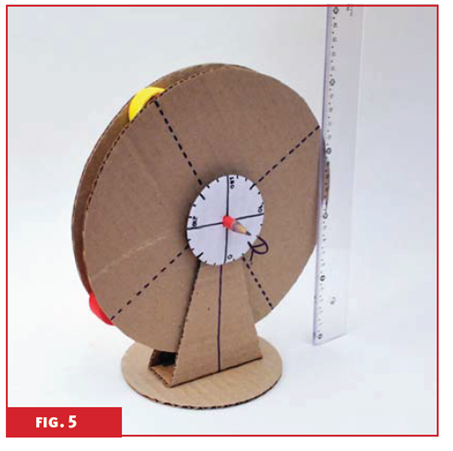
\includegraphics[width=.5\linewidth]{trigonometricas7}
\caption{Fonte: \cite{soares2010}}
\label{}
\end{figure}

Será necessário também o uso de um transferidor para medir os ângulos e uma régua para medir a altura das “cabines”.

Um passageiro entra na cabine quando essa está em seu ponto mais baixo. A partir daí, a roda começa a girar no sentido anti-horário, numa velocidade constante de $20$ graus por segundo. Considere $h = h(t)$ a altura em centímetros da cabine no instante de tempo $t$, medido em segundos.
\begin{enumerate}
\item Calcule a medida do raio da roda gigante e também as alturas mínima e máxima que a cabine pode assumir.
\item Quantos segundos a roda gigante demora para dar uma volta completa?
\item Com o auxílio dos seus colegas, encontre a altura da cabine em cada segundo do movimento da roda gigante até ela completar uma volta. Marque num papel milimetrado os pontos $(t,h(t))$ obtidos.
\item Entre a altura máxima e a altura mínima, há alguma altura intermediária que a cabine atinge mais de uma vez ao longo de cada volta da roda gigante? Quanto mede essa altura intermediária?
\item Determine todos os valores assumidos pela altura h da cabine ao longo de uma volta completa da roda gigante.
\item Observando os pontos marcados no item \titem{c)} e a dinâmica do giro da roda gigante, responda: apesar da velocidade com que a roda gigante gira ser constante, também será constante a taxa de variação da altura da cabine?  
\item Esboce no papel milimetrado uma curva que represente o gráfico de função $h = h(t)$. Como será o gráfico da função para valores de $t$ maiores que $18$ s?
\item Como seria o gráfico de $h = h(t)$ se a velocidade do giro da roda gigante duplicasse, ou seja, se ela demorasse apenas $9$ s para dar uma volta completa? Que alterações podem ser observadas em relação ao gráfico traçado no item \titem{g)}?
\end{enumerate}

\end{task}


\begin{reflection}
Acesse o link de uma roda gigante construída virtualmente no GeoGebra através do seguinte link \url{https://www.geogebra.org/m/g8mnxpgx}

Também é possível visualizar nesse link o gráfico que relaciona a altura da cabine da roda gigante virtual com o tempo.

\begin{figure}[H]
\centering

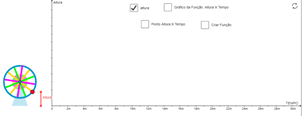
\includegraphics[height=.12\textheight]{trigonometricas8}
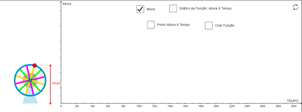
\includegraphics[height=.12\textheight]{trigonometricas9}
\caption{Observação da altura da cabine}

\end{figure}

\begin{figure}[H]
\centering

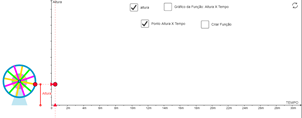
\includegraphics[height=.12\textheight]{trigonometricas10}
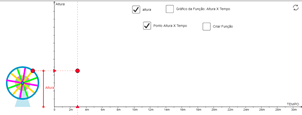
\includegraphics[height=.12\textheight]{trigonometricas11}
\caption{Observação do ponto do plano que associa a $x$ o tempo e a $y$ a altura da cadeira}
\end{figure}

\begin{figure}[H]
\centering

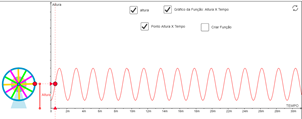
\includegraphics[height=.12\textheight]{trigonometricas12}
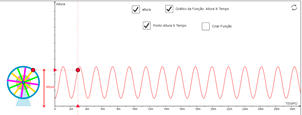
\includegraphics[height=.12\textheight]{trigonometricas13}
\caption{Observação do gráfico da função que associa a $x$ o tempo e a $y$ a altura da cadeira}
\end{figure}

Compare esse gráfico com o gráfico obtido por você e seus colegas na atividade anterior. Como você acha que deveria ser o gráfico se o movimento começasse quando a cabine estivesse no ponto mais alto da roda? E como seria o gráfico se a velocidade com que a roda gigante gira fosse reduzida à metade?
\end{reflection}

\arrange{Fenômenos Periódicos.}
\label{trig-arg1}

O que os fenômenos apresentados nas atividades anteriores têm em comum? Se considerarmos uma situação ideal em que o mesmo fenômeno se repete \textit{exatamente} da mesma maneira ao longo do tempo, podemos dizer que o pêndulo do relógio sempre vai e volta ininterruptamente e que a roda gigante dá várias voltas sem parar. Fenômenos assim são chamados de \textit{periódicos}, ou seja, que se repetem exatamente da mesma forma ao longo do tempo. Ao estudarmos matematicamente as situações que usamos como exemplo aqui, consideramos um modelo. Um \textit{modelo matemático} é uma descrição matemática a partir da observação de algum fenômeno observado no mundo físico. Claro que, ao fazermos essa descrição em termos matemáticos, precisamos fazer algumas restrições e suposições que não necessariamente ocorreram ou ocorreriam de fato no fenômeno observado – mas, com um modelo, é razoável que consideremos essas restrições. Por exemplo, a suposição de que um pêndulo como o da primeira ou da segunda atividade oscila ininterruptamente não ocorre no mundo real: o relógio pode atrasar por algum problema no mecanismo ou até mesmo parar, por exemplo. A roda gigante precisa parar sempre que alguém vai subir ou descer do brinquedo. Mas, as restrições que são feitas para criar o modelo possibilitam que o fenômeno seja estudado, que previsões sejam feitas, além de permitir que outros fenômenos sejam classificados por semelhanças ou diferenças.

Você conhece mais alguns fenômenos periódicos que acontecem na vida?


\begin{figure}[H]
\centering

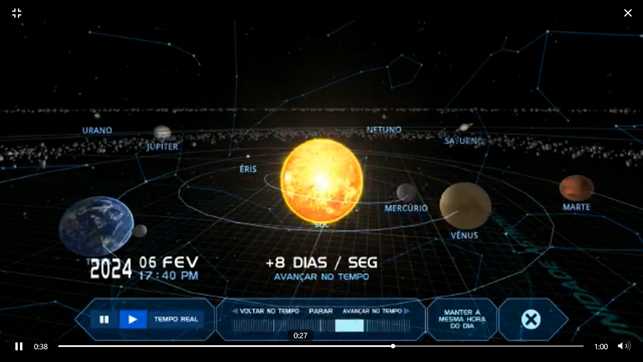
\includegraphics[width=.75\linewidth]{trigonometricas14}
\caption{Fonte: \href{https://www.solarsystemscope.com/}{Solar System Scope}}
\label{}
\end{figure}

O movimento de rotação da Terra em torno de seu próprio eixo é um movimento periódico que demora $24$ h para completar um ciclo (período de $24$ h) e o movimento de translação da Terra ao redor do Sol demora $365$ dias e $6$ h para completar um ciclo (período de $365$ dias e $6$ h).

Nas atividades anteriores você fez os gráficos de funções que representam fenômenos periódicos. Por esse motivo elas também serão chamadas de \textit{funções periódicas}, ou seja, funções cujos valores da imagem se repetem em intervalos fixos. Mais precisamente, uma função $y=f(x)$ é chamada de periódica, se existe algum valor $p$ tal que $f(x)=f(x+p)$, para todos os valores de $x$ tais que $x$ e $x+p$ pertençam ao domínio dessa função. O menor valor positivo de $p$ que satisfizer a essa propriedade será chamado o período dessa função.

Para entender melhor os conceitos que estamos apresentando, vamos discutir um pouco sobre a Atividade \hyperref[trig-ativ1]{“Construindo uma Roda Gigante”}. Nela, você foi orientado a observar o comportamento de uma cabine em específico. Como a roda gigante tem velocidade de rotação constante, o comportamento se repete a cada volta. Isso significa que o gráfico que você gerou para a primeira volta completa da roda gigante vai se repetir exatamente dessa mesma forma por todo o tempo em que a roda gigante permanecer girando. Esse é, portanto, um \textit{fenômeno periódico}.


A velocidade de rotação é de $20$ graus por segundo; logo, uma volta completa ($360^{\circ}$) será alcançada após $18$ segundos. Decorridos os primeiros $18$ segundos de movimento, a roda gigante vai ter dado uma volta completa e a cabine observada terá voltado para sua posição inicial. Matematicamente, podemos escrever que $h(0)=h(18)$. Independentemente da posição ocupada pela cabine no instante $t$, após $18$ segundos a roda gigante dará uma volta completa e a cabine voltará para a mesma posição em que estava quando começamos a marcar o tempo. Matematicamente, essa observação pode ser registrada como  $h(t)=h(t+18)$. É interessante observar que isso é verdade para outros valores: por exemplo, após 36 segundos, a roda gigante terá dado $2$ voltas, portanto $h(t)=h(t+36)$.
De maneira mais geral, considerando um número inteiro positivo k, a roda gigante terá dado $k$ voltas após $18k$ segundos  e, portanto, $h(t)=h(t+18k$), o que indica que essa função é periódica de período $18$, pois esse é o menor valor necessário para que se tenha um ciclo completo do fenômeno observado, ou seja, da roda gigante em movimento.

Mas será que esse é de fato o menor valor para o qual esse ciclo se repete? Note que, por exemplo, quando $t=4{,}5$, a roda gigante terá dado $\frac{1}{4}$	de volta, e portanto, $h(4{,}5)=r$. Após $9$ segundos, a roda gigante terá dado mais $\frac{1}{2}$ volta, assim, a cabine estará a mesma altura que estava no instante $t=4{,}5$, o que indica que $h(4{,}5)=h(4{,}5+9)$. Será que isso significa que $9$ pode ser o período dessa função? Se isso fosse verdade, precisaríamos ter $h(t)=h(t+9)$, para todos os valores $t$ do domínio; no entanto, isso não é verdade, uma vez que no instante $t=0$ a cabine está na posição mais baixa e no instante $t=9$, a roda gigante terá dado $\frac{1}{2}$ de volta e, portanto, a cabine estará na posição mais alta e não de volta ao início, como seria necessário. Note ainda que depois do instante $t=0$, a cabine só voltará para a posição inicial após dar uma volta completa, portanto, após $18$ segundos. Logo, não existe p$<18$ tal que $h(0)=h(0+p)$; ou seja, o período é, de fato $18$.

Repare que, uma vez conhecido o comportamento do gráfico dessa função na faixa $0\leq t\leq18$, também conhecemos o comportamento dela na faixa $18\leq t\leq 36$: será exatamente a repetição do gráfico da faixa anterior, uma vez que a partir de $t=18$ a função se comporta da mesma maneira que se comportava entre $t=0$ e $t=18$. De maneira mais geral, o gráfico na faixa $18k\leq t\leq 18(k+1)$ será uma cópia da faixa do gráfico na faixa $0\leq t\leq 18$.

O período desempenha um papel importante no gráfico de uma função periódica: se conhecermos o desenho do seu gráfico num trecho sobre um intervalo do domínio de comprimento p então podemos esboçar o gráfico inteiro da função, “copiando e colando”{} esse trecho ao longo de todo o domínio.

\begin{figure}[H]
\centering

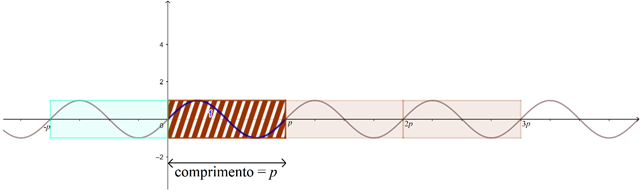
\includegraphics[width=\linewidth]{trigonometricas15}
\end{figure}

A amplitude é outra característica importante quando estudamos uma função periódica. Quando a imagens $f(x)$ de uma função periódica assumirem um valor máximo $M$ e também um valor mínimo m, definimos a \textit{amplitude} de $f$ como sendo $a=\frac{(M-m)}{2}$. Geometricamente, a menor faixa horizontal que contém o gráfico da função $f$ terá largura igual ao dobro da amplitude.

\begin{figure}[H]
\centering

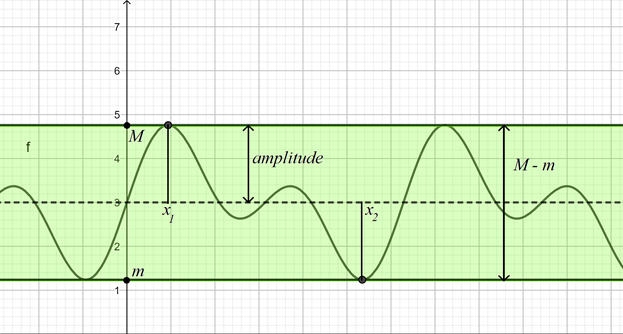
\includegraphics[width=.75\linewidth]{trigonometricas16}
\end{figure}

Na figura a seguir, vemos o gráfico de uma função f definida no intervalo $[-5,5]$, conhecida na literatura como \textit{função dente de serra}.

\begin{figure}[H]
\centering

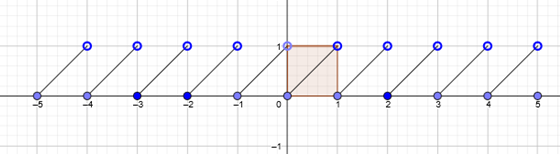
\includegraphics[width=.75\linewidth]{trigonometricas17}
\end{figure}

Podemos perceber que este gráfico é formado por um conjunto de segmentos de reta que são paralelos, sendo que um desses segmentos tem extremidades nos pontos $(0,0)$ e $(1,1)$ e os outros são réplicas desse mesmo trecho do gráfico que se repetem para a esquerda e para a direita. Repare que o ponto $(1,1)$ do segmento replicado é omitido, senão a figura resultante não representaria o gráfico de uma função (Por quê?).

Repare que, para qualquer número $0 < p < 1$, o trecho do gráfico que fica sobre o intervalo $[0, p]$ no eixo $x$ corresponde apenas a uma parte de um desses segmentos de reta, de forma que ao replicarmos essa parte para a esquerda e para a direita, obteríamos uma figura diferente do gráfico da função. Portanto, nenhum número menor que $1 $pode ser o período de $f$. Concluímos que $p =1$ é o \textbf{período} da função.

Como o menor valor e o maior valor assumidos pela imagem são $0$ e $1$ respectivamente, temos que a amplitude é igual $\dfrac{(1-0)}{2}=\dfrac{1}{2}$.

Isso nos mostra que podemos criar uma infinidade de funções periódicas agindo exatamente dessa mesma forma! Podemos definir uma função em um determinado intervalo, por exemplo, $[-2, 0]$, e a partir daí reproduzir por intervalos sucessivos translações horizontais que tenham como fator de translação o mesmo comprimento do intervalo usado como base para criar a função.

\practice{Fenômenos periódicos}
\label{trig-prac1}
\phantom{M}
\vspace{-1em}
\vspace{-\baselineskip}

\begin{task}{Rio Star}
\label{trig-ativ4}

\begin{figure}[H]
\centering

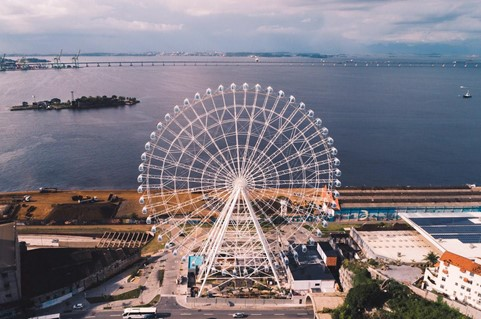
\includegraphics[width=.6\linewidth]{trigonometricas18}
\end{figure}

A Rio Star é a maior roda gigante da América Latina e está localizada na cidade do Rio de Janeiro. Ela tem $88$ metros de altura. A atração turística conta com $54$ cabines climatizadas que podem receber até 8 pessoas cada, totalizando $432$ visitantes que poderão apreciar a vista da Zona Portuária, do Relógio Central, Morro da Providência, Cristo Redentor, Pão de Açúcar, Pedra do Sal, Ponte Rio-Niterói e da Cidade do Samba durante 18 minutos – tempo necessário para a volta completa no brinquedo. (Fonte: \href{https://casavogue.globo.com/LazerCultura/Viagem/noticia/2019/12/rio-star-roda-gigante-do-rio-de-janeiro-inaugura-hoje.html}{Casa Vogue})

Suponha que o ponto mais baixo da roda gigante que qualquer uma das cabines pode atingir se encontra a $3$ metros de altura do chão. Beatriz e Gabriela embarcam em uma das cabines e a partir daí, a roda gigante gira continuamente com a mesma velocidade e dá duas voltas sem parar, finalizando o movimento com a cabine das meninas retornando ao ponto mais baixo.

\begin{enumerate}
\item Qual é o raio da roda gigante?
\item Existe algum momento em que a altura da cabine em relação ao chão será nula? Justifique.
\item Em quais instantes do movimento a cabine estará na mesma altura do centro da roda gigante? E no ponto mais alto da roda? E no ponto mais baixo?
\item Você acha que a altura a que a cabine sobe nos primeiros dois minutos do movimento é a mesma que nos dois minutos seguintes? Justifique sua resposta?
\item No plano cartesiano, plote no plano cartesiano os pontos $(t,h)$ com os dados obtidos no item \titem{c)}, em que $t$ é o tempo e $h$ é a altura da cabine. Em seguida, esboce a curva por meio desses pontos que você acha que representa o gráfico da função altura $h = h(t)$. Compare seu gráfico com o de seus colegas.
\item Qual o período, a amplitude e o conjunto imagem da função $h = h(t)$?
\end{enumerate}
\end{task}

\begin{task}{Construa sua própria função periódica!}
\label{trig-ativ5}

Vamos fazer a nossa própria função periódica?

\begin{enumerate}
\item Usando a malha quadriculada proposta a seguir, defina, a origem, os eixos $Ox$ e $Oy$ e desenhe, usando até $6$ unidades horizontais da malha, uma curva que possa representar o gráfico de uma função, de modo que o ponto inicial da curva tenha mesma altura que o ponto final.
\item Agora, reproduza exatamente esse mesmo trecho por toda a largura da malha, do mesmo jeito como foi feito com a função dente de serra, construindo assim o gráfico de uma função periódica.
\item Qual o período e a amplitude da sua função periódica?
\item Compare o seu gráfico com o de seus colegas. Será que em pelo menos algum deles, você consegue imaginar um contexto real (climática, biológica, doméstica, tecnológica ou outras quaisquer) que ele poderia representar?

\end{enumerate}


\begin{figure}[H]
\centering


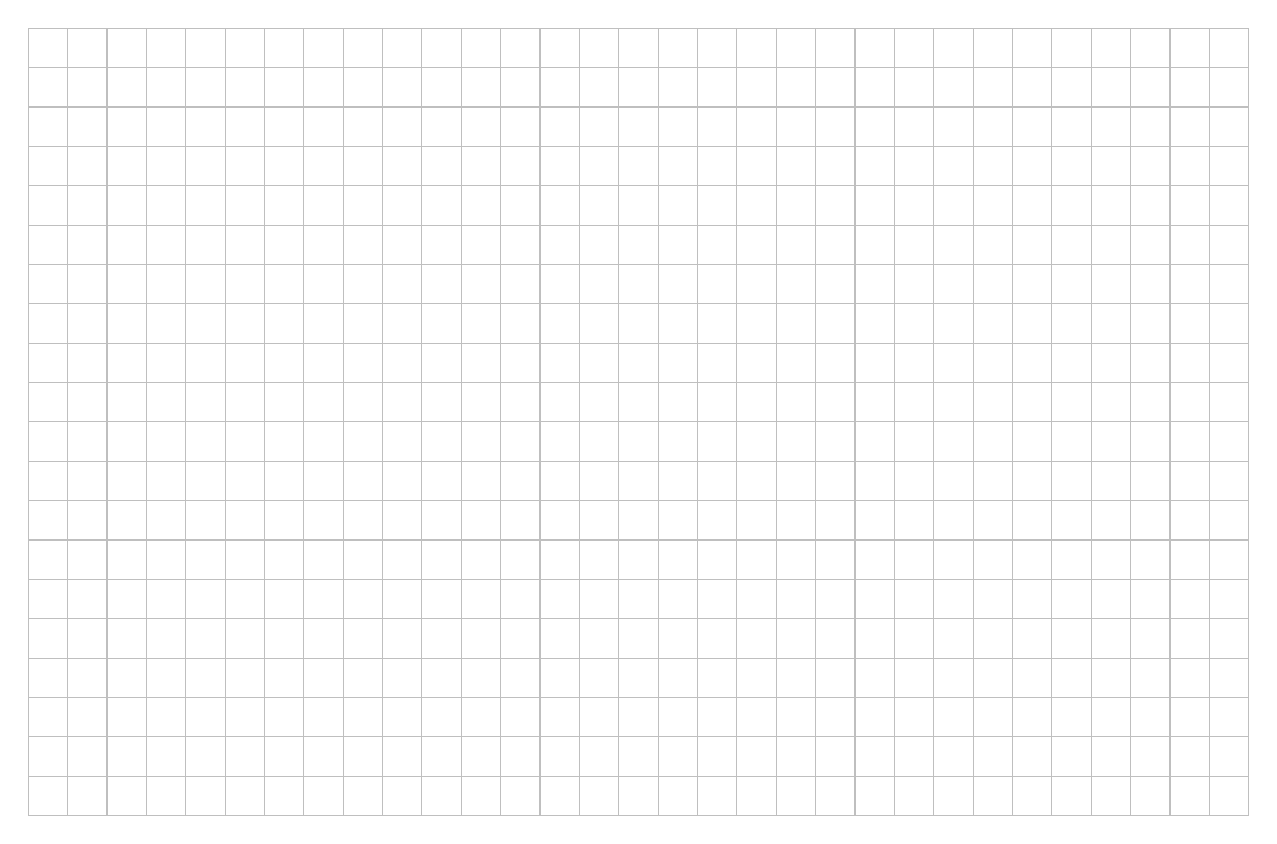
\begin{tikzpicture}
\draw [step=.5,gray!50] (-1.5,-5) grid (14,5);
\end{tikzpicture}

\end{figure}
\end{task}

\clearpage

\begin{task}{Bem estar digital}
\label{trig-ativ6}


Veja um trecho da reportagem a seguir, disponível no endereço \url{http://www.ihu.unisinos.br/78-noticias/591422-uso-excessivo-do-celular-pode-causar-dependencia-e-problemas-psicologicos}


\begin{figure}[H]
\centering

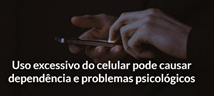
\includegraphics[width=.4\textwidth]{trigonometricas20}

\end{figure}

\begin{quote}

Dados mostram que $12\%$ dos americanos já desenvolveram dependência dos smartphones; psicólogo explica os riscos para a saúde mental.

A reportagem é de Giulia El Halabi, publicada por EcoDebate, 06-08-2019.


Quem nunca pegou o celular apenas para checar mensagens e passou dezenas de minutos – ou até mesmo algumas horas – vidrado na telinha? Esse comportamento cada vez mais comum pode se tornar um vício que já atinge 12\% dos americanos, segundo dados do \textit{Center for Internet and Technology Addiction}.

“O celular ativa continuamente o Sistema de Recompensa, estrutura do cérebro que recebe toda atividade prazerosa. Esse estímulo constante é o que gera dependência, em um processo similar à atuação de drogas ilícitas”, diz o psicólogo e professor do Centro Universitário Internacional Uninter, Ivo Carraro.

O uso abusivo dos smartphones pode gerar transtornos psíquicos, como ansiedade e, posteriormente, depressão. O transtorno já tem um nome: nomofobia, medo de ficar sem o celular. Longe do aparelho, o indivíduo fica ansioso, com a sensação de estar perdendo informações importantes, ou ainda excessivamente entediado.

Outro prejuízo é a dificuldade de sociabilização e isolamento. “Os humanos são seres de linguagem verbal e sociabilidade acentuadas. Quando se comunicam somente por mensagens, que são ‘mudas’, a palavra falada é eliminada e a inépcia social aumenta, agravando quadros depressivos”, explica o professor.

A exposição excessiva ao celular também pode causar insônia. Isso acontece porque a luz azul do aparelho ‘diz’ ao cérebro que ele deve ficar alerta. Assim, a produção de melatonina, o hormônio do sono, é inibida.

\flushright
(Fonte: \href{http://www.ihu.unisinos.br/78-noticias/591422-uso-excessivo-do-celular-pode-causar-dependencia-e-problemas-psicologicos}{Instituto Humanitas Unisinos})
\end{quote}

Como forma de contribuir com os usuários, as plataformas têm disponibilizado algumas ferramentas de registro de acesso aos ambientes mais acessados. Experimente olhar em seu smartphone, nas configurações, se há essa ferramenta – normalmente, o nome é \textit{bem estar digital}.

\begin{figure}[H]
\centering

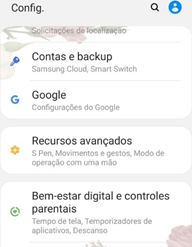
\includegraphics[width=.3\linewidth]{trigonometricas21}
\end{figure}

Por exemplo, alguns registros diários de uso de um aplicativo de mensagens bastante popular no smartphone de uma professora (observando o período de uma semana) estão exibidos a seguir. A primeira informação diz respeito ao número de mensagens recebidas e a segunda informação mostra quantas vezes o aplicativo foi aberto ao longo daquele dia. O dia 13 de agosto foi uma quinta-feira.


\begin{figure}[H]
\centering

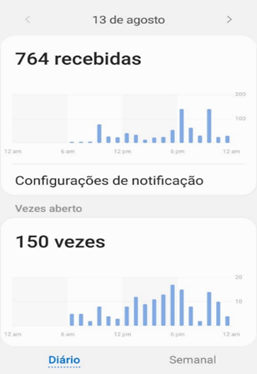
\includegraphics[height=.33\textheight]{trigonometricas22}
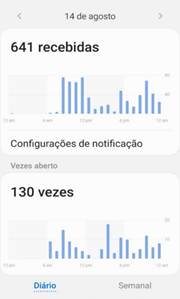
\includegraphics[height=.33\textheight]{trigonometricas23}
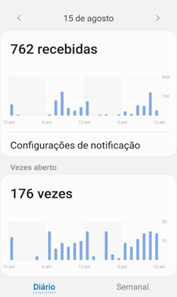
\includegraphics[height=.33\textheight]{trigonometricas24}
\end{figure}

\begin{figure}[H]
\centering

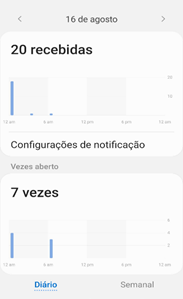
\includegraphics[height=.33\textheight]{trigonometricas25}
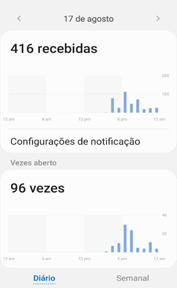
\includegraphics[height=.33\textheight]{trigonometricas26}
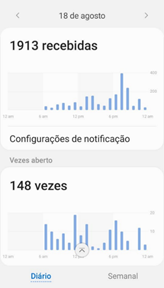
\includegraphics[height=.33\textheight]{trigonometricas27}
\end{figure}

\begin{figure}[H]
\centering

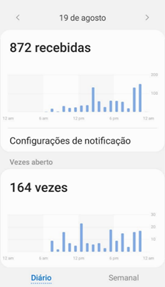
\includegraphics[height=.33\textheight]{trigonometricas28}
\end{figure}
\newpage

\begin{enumerate}
\item Preencha a tabela a seguir com os dados apresentados na figura anterior.

\begin{table}[H]
\centering

\begin{tabular}{|e{.2\linewidth}|e{.2\linewidth}|e{.2\linewidth}|}
\hline
\tcolor{Dia da Semana} & \tcolor{N\super{o} de mensagens recebidas} & \tcolor{N\super{o} de vezes que o aplicativo foi aberto} \tabularnewline
\hline
1 (qui) & & \tabularnewline
\hline
2 (sex) & & \tabularnewline
\hline
3 (sáb) & & \tabularnewline
\hline
4 (dom) & & \tabularnewline
\hline
5 (seg) & & \tabularnewline
\hline
6 (ter) & & \tabularnewline
\hline
7 (qua) & & \tabularnewline
\hline
\end{tabular}
\end{table}

\item Marque num plano cartesiano (físico ou digital) pontos $(x,y)$ correspondendo às duas primeiras colunas da tabela, onde $x$ representa o dia da semana e y o número de mensagens recebidas pela professora naquele dia. Em seguida, construa um segmento de reta ligando o ponto correspondente ao dia 1 ao ponto correspondendo ao dia 2, um segmento de reta ligando o ponto correspondente ao dia 2 ao ponto do dia 3 e assim sucessivamente até chegar ao ponto associado ao dia 7.
\item Faça o mesmo que foi pedido no item \titem{b)}, agora considerando que, nos pares $(x,y)$, $x$ representa o dia da semana e $y$ o número de vezes que para a quantidade de vezes em que a professora abre esse aplicativo.
\item Que observações você pode fazer sobre a rotina dessa professora?
\item As funções com domínio sendo o intervalo $[1,7]$ da reta e cujos gráficos foram esboçados nos itens \titem{b)} e \titem{c)} podem ser ditas periódicas? Se sim, justifique; se não, analise as fotos do enunciado de forma a descobrir ao menos algum padrão de regularidade no comportamento da rotina da professora que poderiam dar ideia de periodicidade.
\item Suponha que os mesmos dados de números de mensagens recebidas e de vezes que o aplicativo foi aberto sejam reproduzidos nos dias seguintes: no dia 8, a professora recebe o mesmo número de mensagens que no dia 1, no dia 9 ela recebe o mesmo número de mensagens que no dia 2 e assim sucessivamente (mesmo raciocínio para o número de vezes que o aplicativo foi aberto). As linhas poligonais construídas ligando pontos consecutivos, como feito nos itens \titem{b)} e \titem{c)}, agora representam gráficos de funções periódicas? Se sim, qual será o valor do período e da amplitude delas?
\item Se você ou alguém de sua família tiver um smartphone com essa função, veja que aplicativos aparecem com registro nessa ferramenta e que parâmetros são exibidos (tempo de tela, número de vezes em que o aplicativo é aberto, número de notificações, entre outros).
\item Colete os dados referentes a algum aplicativo de mensagens e anote, reproduzindo os passos \titem{a)}, \titem{b)}, \titem{c)} e \titem{d)}.

\end{enumerate}

\end{task}


\begin{knowledge}
O som é resultante de uma vibração, que se transmite em meios materiais de propagação, como sólidos, líquidos e gasosos.  Quando uma fonte sonora produz uma vibração, esta é transmitida a todo o meio material que a envolve e em todas as direções. Esta vibração é comunicada aos constituintes mais próximos da matéria, que sucessivamente a transmite aos constituintes seguintes através de choques entre eles.

A vibração de uma fonte sonora causa uma onda no meio de propagação. O som propaga-se por ondas invisíveis: as ondas sonoras ou acústicas. Portanto, o som pode ser descrito através de uma sequência de ondas sonoras, que são ondas de deslocamento, densidade e pressão que se propagam pelos meios compressíveis. Quando uma onda sonora se propaga através de qualquer gás, ocorrem várias compressões e rarefações de pequenos volumes do gás.

\begin{figure}[H]
\centering

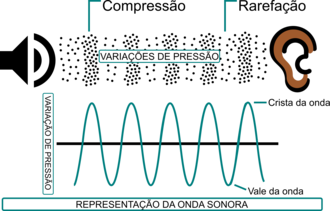
\includegraphics[width=.5\linewidth]{trigonometricas33}
\caption{Fonte: \href{https://pt.wikipedia.org/wiki/Som}{Wikipedia} }
\label{}
\end{figure}

Assista ao vídeo a seguir para compreender melhor o que são as ondas sonoras e como o som se propaga: \url{https://www.youtube.com/watch?v=sEa0dvnqrnw}

\begin{figure}[H]
\centering

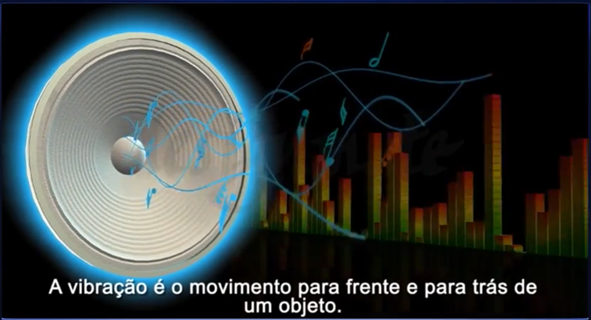
\includegraphics[width=.75\linewidth]{trigonometricas34}
\end{figure}

\needspace{5em}
As ondas sonoras mais simples são representadas por gráficos de um tipo muito específico de função periódica. Em estudos avançados de Física e Matemática constataram que toda onda sonora é gerada a partir de uma combinação dessas ondas sonoras mais simples, ou seja, de funções periódicas.

Podemos enxergar estas ondas? Há um equipamento muito \textit{utilizado} por profissionais da área de elétrica e eletrônica é o osciloscópio, que permite a visualização de formas de ondas eletromagnéticas. Esses dispositivos também são capazes de “ler”{} sinais sonoros, acoplando a eles um microfone.

Faça o \textit{download} em seu celular do aplicativo gratuito \textit{Oscilloscope}. Ele é capaz de captar os sons e reproduzir o que seriam as suas ondas sonoras correspondentes.

\begin{figure}[H]
\centering

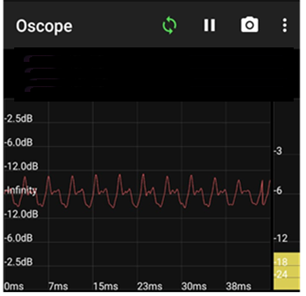
\includegraphics[width=.5\linewidth]{trigonometricas35}
\caption{O aplicativo Oscilloscope. Fonte: Os autore}
\label{}
\end{figure}

\begin{enumerate}
\item Capture com o aplicativo sons em diferentes volumes (clicando no ícone da câmera no topo à direita da tela é possível capturar a imagem da onda sonora). Qual é a diferença nas ondas geradas?
\item Capture com o aplicativo sons graves e agudos. Qual a diferença nas ondas geradas?
\item Procure gerar sons cujas ondas sonoras tenham trechos representados por um gráfico de funções periódicas como a da figura. Explore a relação entre a \textbf{amplitude} e o \textbf{período} da função associada a essa onda.

\end{enumerate}

\end{knowledge}



\needspace{10em}
\begin{knowledge}
O eletrocardiograma (ECG) é um exame médico simples, indolor e rápido, levando em média 3 minutos para fazê-lo, no qual os impulsos elétricos do coração são amplificados e registrados. Em geral, um paciente faz um ECG quando há suspeita de doença cardíaca, mas ele também costuma ser feito como parte de exames físicos de rotina para pessoas de meia-idade e idosas, mesmo que elas não tenham nenhuma evidência de doença cardíaca.

Para realizar o ECG, um examinador coloca eletrodos (sensores redondos e pequenas que aderem à pele) nos braços, pernas e tórax da pessoa. Esses eletrodos medem a magnitude e a direção das correntes elétricas no coração durante cada batimento cardíaco. Os eletrodos são ligados por cabos a uma máquina que produz um registro (traçado) para cada eletrodo. Cada traço mostra a atividade elétrica do coração a partir de ângulos diferentes. No ECG são produzidos esses traços.

A figura a seguir ilustra as ondas associadas às atividades elétricas do coração. O batimento cardíaco começa com um impulso que ativa as câmaras superiores do coração (átrios). A onda P representa a ativação dos átrios. Em seguida, a corrente elétrica flui para as câmaras inferiores do coração (ventrículos). O trecho QRS representa a ativação dos ventrículos. A corrente elétrica, em seguida, espalha-se para trás, ao longo dos ventrículos no sentido oposto. Esta atividade é chamada onda de recuperação, representada pela onda T.



\begin{figure}[H]
\centering

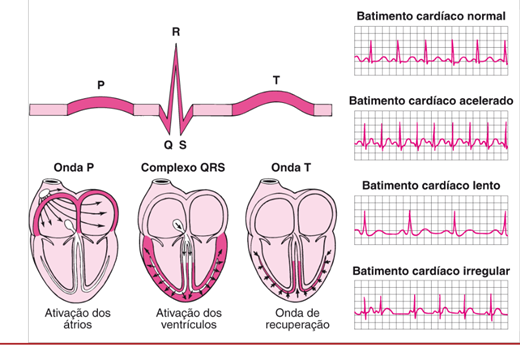
\includegraphics[width=.7\linewidth]{trigonometricas36}
\caption{Fonte: \href{https://www.msdmanuals.com/pt/casa/dist\%C3\%BArbios-do-cora\%C3\%A7\%C3\%A3o-e-dos-vasos-sangu\%C3\%ADneos/diagn\%C3\%B3stico-de-dist\%C3\%BArbios-do-cora\%C3\%A7\%C3\%A3o-e-dos-vasos-sangu\%C3\%ADneos/eletrocardiograma}{Manual MSD}}
\label{eletrocardiograma}
\end{figure}

Como a mecânica do coração se repete constantemente, a sistematização dessas ondas gera uma onda contínua que é impressa ao longo do exame. Em geral, esta onda é representada pelo gráfico de uma função periódica. Quando isto não ocorre, tem-se um indício de arritmia cardíaca, ou seja, um batimento cardíaco irregular.
Mesmo que a onda impressa seja representada por uma função periódica, nem sempre o coração do paciente estará sadio: o batimento cardíaco pode estar mais acelerado ou mais lento do que o normal para uma situação de repouso, o fica visível através do período da função periódica associada ser muito baixo ou muito alto, comparado ao de um batimento cardíaco normal (vide \hyperref[eletrocardiograma]{figura \ref{eletrocardiograma}}).


\end{knowledge}

\explore{O Radiano}
\label{trig-exp2}

\begin{task}{Cobrgindo circunferências com seus raios}
\label{trig-ativ7}

Vamos propor agora uma atividade para você fazer com os seus colegas na sala de aula. Se organizem em duplas ou grupos e sigam os passos a seguir:
\begin{enumerate}[label=\titem{\arabic*.}]
\item Providencie objetos redondos que você possa levar para a sala de aula (rodinhas de carrinho de brinquedo, copos, garrafas, tampas de potes e panela, etc);
\item Use esses objetos para desenhar circunferências numa folha suficientemente grande, contornando-as com um lápis;
\item Determine o centro dessas circunferências. Para isso, tome três pontos sobre a circunferência e trace as mediatrizes de dois segmentos distintos com extremidades nesses pontos. O encontro entre essas mediatrizes é o centro da circunferência;
\item Meça o raio dessas circunferências;
\item Para cada uma das circunferências, corte um pedaço de barbante que tenha essa medida e ajuste-o sobre a circunferência, colando-o no papel.
\end{enumerate}

\begin{figure}[H]
\centering

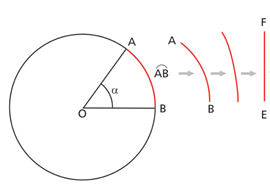
\includegraphics[width=.4\linewidth]{trigonometricas37}
\end{figure}

\begin{enumerate}
\item Qual o nome do objeto geométrico equivalente à parte das circunferências coberta pelo barbante?
\item A partir de cada extremidade dos pedaços de barbante colados sobre cada circunferência, trace dois segmentos que unam as extremidades dos barbantes ao centro de cada circunferência. Meça os ângulos centrais que ficam assim determinados em cada circunferência. Qual a medida do ângulo central encontrada em cada uma delas?
\item Compare a sua resposta do item \titem{c)} com as de outras duplas ou grupos de sua turma. Há algo que você consegue notar nos valores obtidos?
\item Quantas vezes o raio da circunferência cabe no comprimento da mesma?
\item É possível cobrir toda a circunferência com uma quantidade inteira de segmentos com medida igual à do seu raio? Se sim, diga quantos segmentos são necessários; se não, estime o valor da fração do raio do círculo correspondente ao pedacinho que ficou descoberto.
\end{enumerate}
\end{task}


\begin{task}{Ângulos e Arcos de Circunferência no GeoGebra}
\label{trig-ativ8}

Abra o GeoGebra e crie um controle deslizante a variando de $0$ a $10$. Crie o ponto $A$ e construa uma circunferência de centro $A$ com raio $a$. Tome um ponto $B$ sobre a circunferência e construa o segmento $AB$, cujo comprimento ficará registrado na janela da álgebra. Agora, crie um ponto $C$ sobre a circunferência e construa o (menor) arco circular de centro $A$ e extremidades $C$ e $B$, cujo comprimento ficará indicado na Janela da Álgebra.

\begin{enumerate}
\item Usando o GeoGebra, determine a razão $k$ entre o comprimento do arco $BC$ e o raio da circunferência. Movimente o controle deslizante do parâmetro $a$. O que você observa em relação ao valor de $k$?
\item Altere a medida do comprimento do arco $BC$ movendo o ponto $C$ ao longo da circunferência. Qual o intervalo de variação da razão $k$?
\item Movimente $C$ de forma que o comprimento do arco $BC$ fique igual ao comprimento do raio da circunferência. Qual o valor da razão $k$ nesse caso? Movimente o controle deslizante novamente e registre o que você observa.
\item Construa e meça o ângulo central ${B\hat{A}C}$ e modifique a unidade de medida para \textit{“radianos}”. Movimente o ponto $C$ sobre a circunferência. O que você pode observar em relação ao valor de $k$ e a medida do ângulo central da circunferência em radianos?
\item Movimente o controle deslizante a e observe o valor da razão $k$.
\item Reproduza a atividade, agora com uma circunferência que tenha um raio fixo e igual a $1$. Comente como ficam os valores de $k$ e do ângulo ${B\hat{A}C}$.
\end{enumerate}

\end{task}

\arrange{O Radiano}
\label{trig-arg2}

Na atividade \hyperref[trig-ativ7]{Cobrindo circunferências com seus raios}, você pôde observar que, mesmo que variemos o raio da circunferência, o ângulo central (com vértice no centro da circunferência) determinado por um arco da circunferência que tem comprimento igual à medida do raio é o mesmo. Além disso, também foi possível verificar que cabem sobre a linha da circunferência $6$ “pedaços”{} inteiros de barbante com o comprimento igual ao raio da circunferência, faltando um arco cujo comprimento é menor que o comprimento do raio da circunferência em questão.

Na segunda atividade – \hyperref[trig-ativ8]{Ângulos e Arcos de Circunferência no GeoGebra} – você pôde observar que a razão entre o comprimento de um arco qualquer na circunferência e o seu raio varia entre $0$ e valores menores que $6{,}3$ – ou seja, isso indica que o raio da circunferência “cabe”{} sobre o seu contorno pouco mais de $6$ vezes inteiras. Mas exatamente, quantas vezes será que o raio de uma circunferência cabe sobre o seu contorno?

Para determinar esse valor, vamos nos lembrar que, no Ensino Fundamental, você aprendeu que o comprimento $C$ de uma circunferência de raio $r$ é $C=2\pi r$. A operação que nos permite verificar quantas vezes uma grandeza “cabe”{} em outra de mesma natureza é a divisão; então, como queremos verificar quantas vezes o raio cabe na circunferência, vamos dividir o comprimento da circunferência pelo raio. Temos então:
\begin{equation*}
\frac{2\pi r}{r}=2\pi.
\end{equation*}

Isso quer dizer que o raio de uma circunferência cabe sobre o seu contorno $2\pi$ vezes – o que é coerente com o que encontramos na atividade \hyperref[trig-ativ8]{Ângulos e Arcos de Circunferência no GeoGebra} ou ainda na atividade \hyperref[trig-ativ7]{Cobrindo circunferências com seus raios}. Tomando para   o valor aproximado de $3{,}14$ (lembrando que esse é uma aproximação, na verdade,$\pi$ é um número irracional!), encontramos $2\cdot\pi\cong2\cdot3{,}14=6{,}28$, ou seja, pouco menos do que $6,3$. E observe: esse resultado não depende do raio da circunferência!

O que estamos fazendo aqui é uma ação de \textbf{\textit{medir} arcos de circunferências} (e seus respectivos ângulos centrais), mas usando o \textbf{\textit{raio da circunferência como unidade de medida}} e não os já conhecidos graus, que remetem ao ângulo central da circunferência que determina o arco que desejamos medir. A unidade de medida de arcos provenientes dessa ação é o \textit{radiano}. Escrevemos $\rad$ para denotar esta nova unidade medida. Então, o radiano é uma unidade de medida de arcos tal que $2\pi \rad$ é a medida do arco que cobre completamente a circunferência, sem sobreposições. Assim sendo, podemos estabelecer uma correspondência entre a nossa já conhecida unidade de medida de arcos em graus e a nova unidade radianos: como o arco de uma volta inteira mede, em graus, $360^{\circ}$, então podemos escrever que:
\begin{equation*}
360^{\circ}=2\pi\rad
\end{equation*}

Dividindo os dois lados da igualdade por $2$, teremos de forma mais simplificada que $180^{\circ}=\pi \mathrm{rad}$. Podemos usar essa relação para poder ler a medida de qualquer arco em graus ou em radianos, convertendo de uma à outra sempre que necessário. Em particular, a medida em graus de um arco cujo comprimento é de $1\rad$ (um arco cujo comprimento é exatamente $1$ raio) pode ser determinada dividindo-se ambos os termos na igualdade acima por $\pi$:
\begin{equation*}
180^{\circ}=\pi \rad\therefore\frac{180^{\circ}}{\pi}=\frac{\pi}{\pi} \rad\therefore1 \rad=\frac{180^{\circ}}{\pi}
\end{equation*}

\begin{observation}{}
É interessante observar que, ao tratar dessas duas unidades de medida, estamos percebendo duas características importantes do arco: a medida do ângulo central que o determina sobre a circunferência e a quantidade de vezes que o raio da circunferência cabe sobre aquele arco. Quando desejamos nos remeter à medida do arco correspondente ao ângulo central, a medida em graus é a mais esclarecedora; por outro lado, quando desejamos indicar quantos raios cabem no comprimento do arco, então a medida em radianos é a mais adequada. E note que podemos facilmente transitar de uma à outra a partir do uso da relação $180^{\circ}=\pi\rad$.
\end{observation}


Para podermos ter uma boa ideia do que estamos tratando, vamos considerar dois relógios analógicos: o relógio de Meca, dito o maior do mundo, que tem $4$ faces com $43$ metros de diâmetro em cada face e um relógio de pulso comum, que tem em torno de $3$ cm de diâmetro.

\begin{figure}[H]
\centering

\begin{minipage}{.45\linewidth}
\begin{figure}[H]
\centering

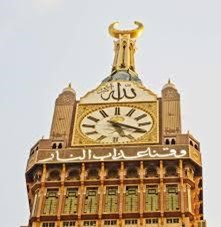
\includegraphics[height=175bp]{trigonometricas38}
\caption{Fonte: \href{https://gigantesdomundo.blogspot.com/2012/11/o-maior-relogio-do-mundo.html}{Gigantes do Mundo}}
\label{}
\end{figure}
\end{minipage}
\hspace{2em}
\begin{minipage}{.45\linewidth}
\begin{figure}[H]
\centering

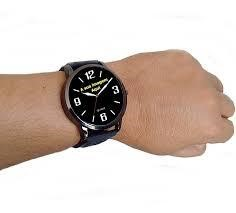
\includegraphics[height=175bp]{trigonometricas39}
\caption{Fonte: \href{https://produto.mercadolivre.com.br/MLB-1160291326-relogio-pulso-personalizado-com-foto-imagem-logo-promoco-_JM}{Mercado Livre}}
\label{}
\end{figure}
\end{minipage}
\end{figure}

Vamos considerar que os dois relógios estão marcando corretamente as horas, sem atrasar nem adiantar, e que ambos estejam marcando exatamente $3$ h – ou seja, o ponteiro pequeno aponta para o número $3$ e o ponteiro grande para o número $12$. Vamos observar os arcos determinados nos dois relógios pelas semirretas que têm origem no centro dos relógios e que passam pelo $12$ e pelo $3$, respectivamente.

\begin{figure}[H]
\centering

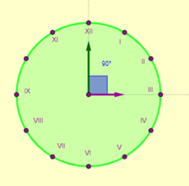
\includegraphics[width=.35\linewidth]{trigonometricas40}
\hspace{2em}
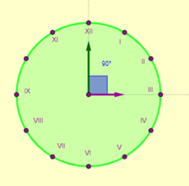
\includegraphics[width=.35\linewidth]{trigonometricas40}
\caption{Disponível em: \url{https://www.geogebra.org/m/gTMSvJTB}}
\label{}
\end{figure}

Nos dois relógios, a medida do arco de extremidades $C$ e $E$ tem a medida de $90^{\circ}$ - essa é a medida angular desse arco, pois remete à medida do ângulo central de vértice $D$ que mede também $90^{\circ}$. Por outro lado, evidentemente, a medida do \textit{comprimento} do arco de extremidades $C$ e $E$ é diferente nos dois relógios: no relógio de pulso, de diâmetro $3$ cm (e raio $1{,}5$ cm), o comprimento desse arco será de $C=\frac{(2\cdot\pi\cdot1{,}5}{4}=\frac{3}{4}\pi$ cm, ou seja, aproximadamente $2{,}35$ cm . Por outro lado, no relógio de Meca com $43$ m de diâmetro, temos $21{,}5\text{ m } = 2150$ cm de raio e então o arco $CE$ terá comprimento  
\begin{equation*}
C=\dfrac{2\cdot\pi\cdot2.150}{4}=1.075\pi\cong3375{,}5\text{ cm}.
\end{equation*}
Porém, a medida em radianos do arco $CE$ em ambos os relógios será a mesma! Lembre-se: medir um arco em radianos significa que queremos saber quantas vezes o raio da circunferência cabe naquele arco. No relógio de pulso, a medida em radianos de CE será o quociente entre a medida do seu comprimento pelo raio da circunferência, isto é, $\dfrac{\frac{3}{4}\pi}{1{,}5}=\frac{\pi}{2}\rad$, enquanto que no relógio de Meca será $\dfrac{1.075\pi}{2.150}=\dfrac{\pi}{2}\rad$. Repare que, segundo a regra de conversão $108^{\circ}=\pi\rad$, estabelecida entre graus e radianos dividindo ambos os lados da igualdade por $2$, obtemos $90^{\circ}=\frac{\pi}{2}\rad$. Em particular, arcos correspondendo a ângulos retos medem $\frac{\pi}{2}\rad$.

\clearpage
\practice{O Radiano}
\label{trig-prac2}

\begin{task}{Medindo ângulos centrais em nosso planeta}
\label{trig-ativ9}

Um dos resultados mais fascinantes que já existiram na História da Matemática é decorrente do experimento realizado pelo matemático e astrônomo grego Eratóstenes. Estudando o comportamento das sombras de varetas nas cidades Alexandria e Syene (Assuã, nos dias atuais) ao meio dia, ele não só conseguiu perceber que a superfície da Terra não era plana como conseguiu calcular, com uma precisão surpreendente, o comprimento de uma volta completa ao redor da Terra!

Eratóstenes sabia que a distância entre as cidades de Alexandria e Syene era aproximadamente igual a $800$ km. Percebeu também que ao meio dia, o sol estava a pino em Syene de forma que nesse horário, podia-se ver o sol completamente refletido no interior do poço. Além disso, às $12$ h, nenhuma sombra era formada pelas colunas daquela cidade. O mesmo não ocorria em Alexandria: ao meio dia, uma vareta colocada de pé no chão apresentava uma sombra substancial e com ela, Eratóstenes conseguiu provar que o arco sobre a superfície da Terra, que compreende as cidades de Alexandria e Assuã media cerca de $\frac{\pi}{25}\rad$ ($7{,}2$ graus) e que corresponde ao ângulo central $\hat{A}$ da \hyperref[zenite]{figura \ref{zenite}}:

\begin{figure}[H]
\centering

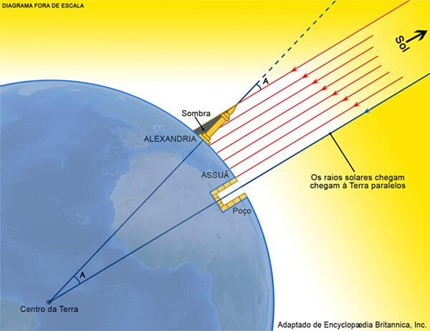
\includegraphics[width=.65\linewidth]{trigonometricas42}
\caption{Costa, J. R. V. Eratóstenes e a circunferência da Terra. \href{https://www.zenite.nu/eratostenes-e-a-circunferencia-da-terra/}{Astronomia no Zênite}, jul 2000.}
\label{zenite}
\end{figure}

Eratóstenes utilizou a seguinte regra de três para calcular o comprimento de uma volta completa ao redor da Terra:


\begin{equation*}
\begin{array}{ccc}
\frac{\pi}{25} \rad & \adjustbox{valign=c}{\tikz \draw (0,0) -- (1.5,0);} & 800 \text{ km} \\
2\pi\rad & \adjustbox{valign=c}{\tikz \draw (0,0) -- (1.5,0);} & C 
\end{array}
\end{equation*}

Resolvendo a regra de três, obtemos $C = 40.000$ km. Utilizando instrumentos tecnológicos muito mais avançados dos quais dispunha Eratóstenes, hoje se sabe que o comprimento de uma volta completa na Terra é de $40.072$ km, ou seja, o erro de cálculo do matemático grego foi de menos de $100$ km! O vídeo a seguir, apresenta parte de um episódio famosa série Cosmos, e narra com mais detalhes a ideia do experimento de Eratóstenes.

\begin{figure}[H]
\centering

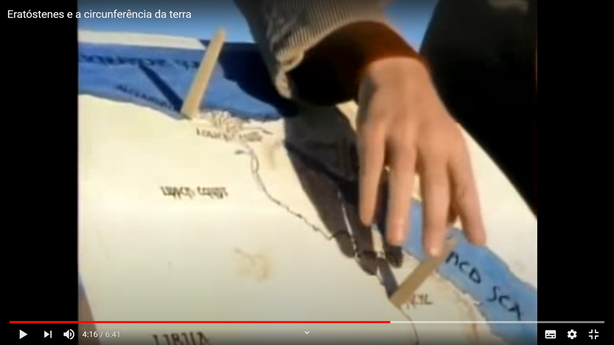
\includegraphics[width=.5\linewidth]{trigonometricas43}

\caption{Acesse pelo link: \url{https://www.youtube.com/watch?v=fu9Z7YuXLVE}}
\end{figure}

Vamos utilizar o raciocínio de Eratóstenes, com o auxílio do Google Earth para medir arcos em graus e radianos, limitados por duas cidades brasileiras! Baixe e instale no seu smartphone o aplicativo Google Earth.


\begin{figure}[H]
\centering

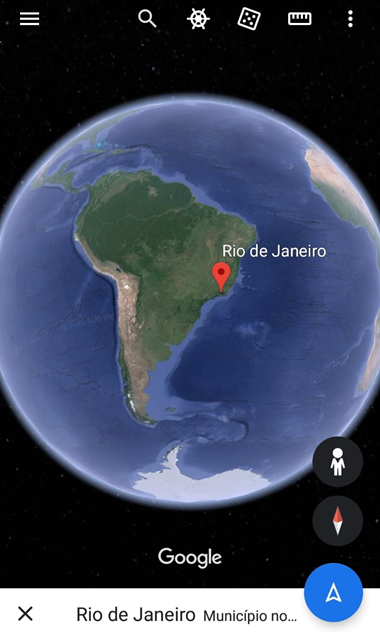
\includegraphics[height=.3\textheight]{trigonometricas44}
\end{figure}

\begin{enumerate}
\item Use a ferramenta medir para encontrar uma aproximação para distância, ao longo do globo terrestre, entre as capitais Rio de Janeiro e Belo Horizonte.
\item Usando o fato que uma volta completa na Terra tem $40.072$ km, determine a medida aproximada do valor do arco (em radianos) sobre a superfície da Terra que liga as duas capitais do item \titem{a)}.
\item Reproduza os itens \titem{a)} e \titem{b)} para a cidade onde você mora e qualquer outra cidade de sua escolha no Brasil.
\end{enumerate}
\end{task}

\explore{Círculo Trigonométrico e a Função de Euler}
\label{trig-exp3}

\begin{task}{Carrinho VertiGo}
\label{trig-ativ10}

\begin{quote}

Pesquisadores da Disney Research, em parceria com o Instituto Federal de Tecnologia de Zurique, demonstraram esta semana um carrinho de quatro rodas capaz de escalar paredes e andar normalmente em superfícies verticais.
À primeira vista, parece um brinquedo, mas, segundo os criadores, a tecnologia pode ampliar os limites de exploração para equipamentos robóticos. Batizado como VertiGo, o carrinho é “capaz de mover em uma parede rapidamente e com agilidade”, informam os pesquisadores. Para realizar a façanha, ele possui duas hélices propulsoras móveis que fornecem o impulso necessário para o início da escalada e, depois, mantém o VertiGo junto à parede.”

\flushright
Fonte: \href{https://gizmodo.uol.com.br/o-novo-robo-da-disney-escala-paredes-como-uma-lagartixa/}{Gizmodo}
\end{quote}


\begin{figure}[H]
\centering

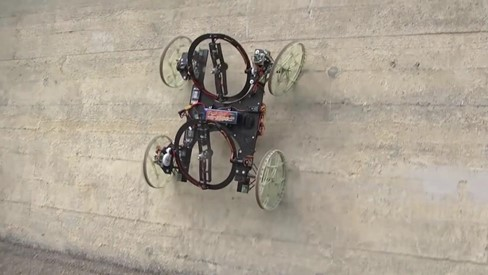
\includegraphics[width=.7\linewidth]{trigonometricas45}
\end{figure}

Neste link é possível ver o VertiGo em ação: \url{https://www.youtube.com/watch?v=KRYT2kYbgo4}


Suponha que foi colado um pequeno selo em uma das rodas do VertiGo. O carrinho começará a descer em um paredão vertical bem alto, seguindo um caminho reto e paralelo ao paredão. Ele começa o movimento “colado”{} ao paredão, quando o selo está em contato com o mesmo. Conforme o carrinho vai descendo, o selo se movimenta conforme o giro da roda. A figura abaixo ilustra o movimento realizado por essa roda ao descer o paredão e os pontos $A_1$, $A_2$ e $A_3$ ilustram posições do selo ao longo do movimento. Suponha que o raio da roda seja de $1$ dm

\begin{figure}[H]
\centering

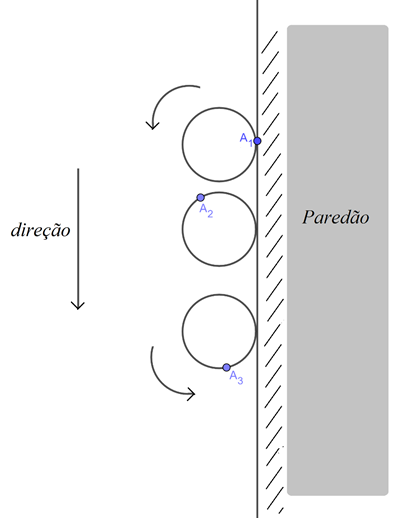
\includegraphics[width=.375\linewidth]{trigonometricas46}
\caption{Fonte: Adaptado de \cite{ekici2010}}
\label{trigonometrica46}
\end{figure}

\begin{enumerate}
\item Indique a posição do selo na circunferência da roda quando o VertiGo tiver descido as seguinte distâncias:

$0\text{ dm}, 1\text{ dm}, 2\text{ dm}, \frac{3}{2}\text{ dm}, \frac{\pi}{2}\text{ dm}, \pi\text{ dm}, 3\pi\text{ dm}, 2\pi\text{ dm}, 7\text{ dm}, 4\text{ dm}$
\item Suponha que, do ponto de repouso do VertiGo, agora ele irá \textbf{subir} parte do paredão. Usando a mesma vista lateral dada pela \fref{trigonometrica46}, qual será a posição do sela para as mesmas medidas do item \titem{a)}?
\end{enumerate}


\end{task}

\begin{task}{"Abraçando"{} um círculo com uma reta}
\label{trig-ativ11}

Observe a imagem a seguir e responda às perguntas:
\begin{figure}[H]
\centering

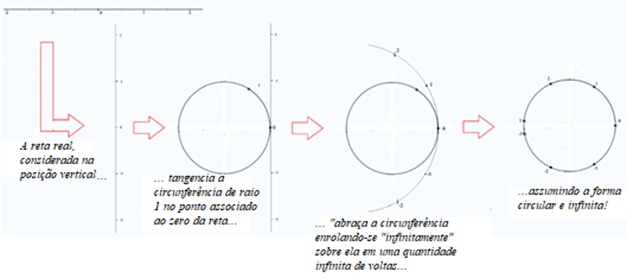
\includegraphics[width=.9\linewidth]{trigonometricas48}
\end{figure}

\begin{enumerate}
\item Quantos pontos da circunferência estarão “cobertos”{} pelo número real $1$?
\item A cada ponto da circunferência, quantos números reais ficam associados?
\item Considerando o ponto $A$ na circunferência sobre o qual encontra-se o número real $1$. Qual o próximo número real positivo que também estará localizado em $A$? E qual será o primeiro número negativo associado a $A$?
\item Se reproduzimos a construção exibida acima usando, em lugar da reta real, o intervalo $[-5,5]$ em uma circunferência de raio $2$, tangenciando esta circunferência no ponto $0$ do intervalo, qual será a medida do menor arco encontrado entre os pontos da circunferência associados a $-5$ e $5$?
\end{enumerate}
\end{task}

\arrange{Círculo Trigonométrico e a Função de Euler}
\label{trig-arg3}

Nas atividades \hyperref[trig-ativ10]{\textit{Carrinho VertiGo}} e \hyperref[trig-ativ11]{\textit{"Abraçando"{}  um círculo com uma reta}} você aprendeu que é possível associar números reais a pontos de uma circunferência de raio $1$. Considere que no plano tem-se um sistema de coordenadas cartesianas, no qual $C^1$ representa a circunferência de centro na origem e raio $1$. Repare que $A = (1,0)\in C^1$ pois esse ponto tem distância $1$ para a origem. A \textit{Função de Euler}, que será denotada pela letra $E$, é uma ferramenta matemática que permite corresponder formalmente qualquer número real a um ponto de $C^1$. Definimos $E:R\to C^1$,  da seguinte maneira: dado qualquer número real $t > 0$, construiremos um arco de comprimento $|t|$ na circunferência  $C^1$, com uma de suas extremidades no ponto $A$ e a outra extremidade num ponto $E(t)$ percorrendo $C^1$ no sentido contrário aos ponteiros do relógio (anti-horário). Se $t < 0$ fazemos o mesmo procedimento, porém percorrendo a circunferência em sentido horário. Finalmente, se $t = 0$, definimos $E(0) = A$.

\begin{minipage}{.45\linewidth}
\begin{figure}[H]
\centering

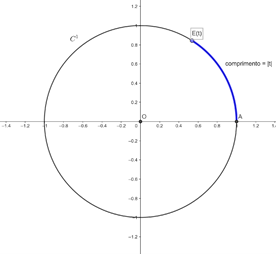
\includegraphics[width=\linewidth]{trigonometricas50}
\caption{$E(t)$ para $t>0$}
\label{}
\end{figure}
\end{minipage}
\begin{minipage}{.45\linewidth}
\begin{figure}[H]
\centering

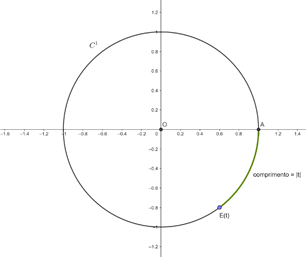
\includegraphics[width=\linewidth]{trigonometricas51}
\caption{$E(t) \text{ para } $t<0}
\label{}
\end{figure}
\end{minipage}

Repare que eventualmente, o valor de $|t|$ pode ser maior que a medida do comprimento da circunferência $C^1$ . Se isto ocorrer, o arco de extremidades $A$ e $E(t)$ será construído de forma que se percorrerá a linha da circunferência dando mais que uma volta em torno da origem do plano cartesiano: por exemplo, se $t=-4\pi$, então, como $C^1$ tem comprimento $2\pi\cdot1=2\pi$, $E(t)$ será obtido construindo um arco partindo de $A$ e fazendo-se um percurso de $|-4\pi |=4\pi$ unidades ao longo de $C^1$ no sentido horário, o que corresponde exatamente a dar umas voltas completas na circunferência, finalizando o percurso em $A$. Logo, $E(-4\pi)=A$. Por outro lado, para encontrar $E(7\pi)$, começamos percorrendo $7\pi$ unidades de comprimento ao longo de $C^1$ , mas agora em sentido anti-horário. O percurso termina no ponto $(-1,0)$ pois $7\pi=3\cdot(2\pi)+\pi$, o que corresponde a dar $3$ voltas em $C^1$ a partir de $A$ no sentido anti-horário e depois percorrer mais meia volta. Logo, $E(7\pi) = (-1,0)$.

A dinâmica do cálculo de imagens pela Função de Euler motiva a definição do \textbf{círculo (ou ciclo) trigonométrico} que consiste essencialmente em três ingredientes: circunferência de raio unitário, sistema de eixos cartesianos e orientação. Vamos falar um pouco sobre cada um deles.

\paragraph{Circunferência de raio unitário}

Vimos na seção “O radiano”{} que a medida de um arco em radianos indica a quantidade de vezes que o raio da circunferência na qual o arco está contido “cabe”{} sobre esse arco, ou seja, a medida angular do arco é o resultado da razão entre o comprimento do arco e o raio da circunferência que contém esse arco. Lembre-se que a medida em radianos de um arco em uma circunferência é calculada através do quociente entre o comprimento do arco e o raio. Esse cálculo fica mais fácil quando o raio mede $1$ unidade, o que nos dá uma equivalência direta entre $C^1$ o comprimento do arco e a medida angular em radianos desse arco. Então, considerar arcos em uma circunferência de raio unitário traz a vantagem de termos medidas de mesmo valor para as medidas angular (relacionada ao ângulo central, à abertura do arco) e linear (relacionada ao comprimento do arco).

\paragraph{Sistema de eixos cartesianos}

O sistema de eixos cartesianos é o sistema com um par de retas perpendiculares orientadas e graduadas, em cuja interseção se localiza o ponto de coordenadas $(0,0)$, denominado \textit{origem do sistema de eixos cartesianos}. A associação entre o sistema de eixos cartesianos e a circunferência de raio unitário nos possibilitará associar coordenadas aos pontos sobre a circunferência.

\paragraph{Orientação}

A circunferência que representa o círculo trigonométrico é orientada, o que indica que há um ponto tomado como origem e uma orientação que atribui um sentido positivo (sentido anti-horário) e um sentido negativo (sentido horário) para os arcos tomados sobre essa circunferência. A seguir podemos ver uma imagem que representa o círculo trigonométrico e seus pontos notáveis.

\begin{figure}[H]
\centering

\includegraphics[width=.75\linewidth]{trigonometricas52}
\end{figure}

A partir do momento em que conseguimos associar comprimentos com arcos no círculo trigonométrico, já podemos pensar em associar números reais ao círculo trigonométrico. Um arco de comprimento 2, por exemplo, seria um arco de $2 \rad$ --– mas onde ele começa? Onde acaba? E o arco de $-2\rad$, onde o marcamos?

Determinar a origem do círculo trigonométrico como sendo o ponto $(1,0)$ e estabelecer o sentido positivo como o anti-horário e negativo como o horário torna essa missão mais simples. Um arco de $2\rad$ tem origem em $(1,0)$ e estende-se por um comprimento igual a $2$ unidades no sentido anti-horário. E o arco de $-2 \rad$? Esse arco também tem origem em $(1,0)$, mas estende-se com comprimento $2$, mas no sentido horário do círculo, pois é negativo. Na figura a seguir vemos esses arcos.

\begin{figure}[H]
\centering

\includegraphics[width=.39\linewidth]{trigonometricas53}
\end{figure}

Por sua vez, o número zero será associado a um “arco”{} que consiste em um único ponto, a saber, a origem $(1,0)$ do círculo trigonométrico.

Vamos generalizar essas ideias? Na figura a seguir, o ângulo ${B\hat{O}A}$ tem medida $\alpha$, em graus. A \textit{medida} do arco $AB$ será  $\frac{\alpha}{360^{\circ}}\cdot2\pi\rad$. A razão $\frac{\alpha}{360^{\circ}}$ indica que parte da circunferência inteira (de comprimento $2\pi$ pois o raio é $1$) é ocupada pelo arco $AB$. Se $\alpha$ é dado em radianos, então a medida do arco $AB$ será, da mesma forma que vimos acima, $\frac{\alpha}{2\pi}\cdot2\pi\rad$ , ou seja, é $\alpha$.

\begin{figure}[H]
\centering

\includegraphics[width=.35\linewidth]{trigonometricas54}
\end{figure}

Por essa razão é tão interessante usar a unidade radianos para medir arcos e ângulos em trigonometria: esta unidade é flexível e pode ser entendida tanto como medida angular quanto como medida linear.

\subsection{Arcos Côngruos}

Agora vamos pensar em outra questão: qual é o maior arco que pode ser tomado no círculo  trigonométrico? E qual é o menor? Eles existem? A resposta é \textbf{não}. Basta considerarmos que um arco pode dar um número arbitrário de voltas em torno do círculo trigonométrico, gerando o que chamamos de \textit{arcos côngruos}, ou seja, arcos que têm a mesma origem e a mesma extremidade, mas que diferem pelo número de voltas inteiras dadas no círculo trigonométrico.

Considere, como exemplo, um arco $AB$ de medida $\frac{\pi}{6} \rad$, por exemplo, e outro arco $AC$ de medida $\frac{13\pi}{6}$ rad. Como, 
\begin{equation*}
\frac{13\pi}{6}=\frac{\pi}{6}+\frac{12\pi}{6}=\frac{\pi}{6}+2\pi,
\end{equation*}
então temos que o arco $AC$ tem a mesma extremidade do arco AB, ou seja, os pontos $B$ e $C$ são coincidentes. Geometricamente, o arco orientado $AC$ é construído traçando o arco $AB$ e em seguida, a partir de $B$, se dá uma volta completa no círculo no sentido positivo, de forma que $C$ coincida com o ponto $B$. Arcos que têm esta característica são aqueles que chamamos de arcos côngruos. Outros arcos côngruos ao arco $AB$ seriam $\frac{25\pi}{6} \rad$ ($2$ voltas inteiras e mais  $\frac{1}{12}$ de volta, no sentido positivo), $\frac{11\pi}{6}\rad$ ($\frac{11}{12}$ de volta no sentido negativo) ou ainda $-\frac{23\pi}{6}\rad$ (uma volta inteira e mais $\frac{1}{12}$ de volta no sentido negativo), entre \textit{infinitas} outras possibilidades.

Para um arco $AB$ medindo $x\rad$, a \textit{expressão geral da medida de um arco côngruo} a $AB$, é dada por, $x+2k\pi$ onde $k$ é um número inteiro. Quando dois arcos de medidas $x$ e $y$ são côngruos, escrevemos $x\equiv y$. Então, segundo essa notação, temos $x\equiv x+2k\pi$. Se a medida $x$ do arco $AB$ for feita em graus ao invés de radianos, teremos que todos os arcos côngruos a $AB$ terão medida em graus dadas por $x+360^{\circ}\cdot k$ com $k$ inteiro. A menor medida $x$ de um arco côngruo a $AB$ (em graus ou radianos) positivo, será chamada de \textit{menor determinação} positiva do arco $AB$ (ou \textit{primeira determinação }positiva).

\practice{Círculo Trigonométrico e a Função de Euler}
\label{trig-prac2}

\begin{task}{Círculo trigonométrico no GeoGebra}
\label{trig-ativ12}

Abra uma tela nova no GeoGebra e exiba os eixos coordenados. Construa os pontos $A(0,0)$ e $B(1,0)$ e construa o círculo de centro $A$ que passa por $B$.
\begin{enumerate}
\item Qual o raio dessa circunferência?
\item Quais os pontos de interseção entre a circunferência e os eixos coordenados? Quanto mede cada um dos arcos compreendidos entre esses pontos?
\item Os pontos que se localizam na circunferência cujas coordenadas são positivas são pontos que estão no $1$\super{o} quadrante. Faça uma figura indicando onde estão esses pontos. Da mesma forma, indique onde se localizam os que estão no $2$\super{o} quadrante (abscissa negativa e ordenada positiva), no $3$\super{o} quadrante (coordenadas negativas) e no $4$\super{o} quadrante (abscissa positiva e ordenada negativa).
\clearpage

\item Considere a reta real “enrolada”{} na circunferência conforme vimos no exercício anterior, com a mesma unidade dos eixos coordenados. Em que quadrante fica o número real $1$? E o número real $-1$? E o número real $\pi$? E o número real $\sqrt{2}$?
\item Marque um ponto $C$ sobre a circunferência de forma que o ângulo $B\hat{A}C$ meça $60^{\circ}$. Que número real está associado ao ponto C?
\end{enumerate}
\end{task}

\begin{task}{Quantas voltas tem o arco e qual é o seu quadrante?}
\label{trig-ativ13}

Considerando os quadrantes no círculo trigonométrico, indique em qual quadrante se localiza a extremidade de cada arco indicado a seguir. Informe também qual o número de voltas completas em torno do círculo é possível se dar com cada um desses arcos.

\begin{enumerate}
\item $8{,}5\rad$
\item $-1{,}37\rad$
\item $\dfrac{\sqrt{2}}{5}\rad$
\item $-0{,}03\rad$
\item $17\dfrac{3}{5}\rad$
\item $-20{,}42\rad$
\end{enumerate}
\end{task}

\begin{task}{Marcando ângulos no círulo trigonométrico}
\label{trig-ativ14}

Dê a menor determinação positiva dos arcos a seguir e indique sua expressão geral dos arcos.
\begin{enumerate}
\item $1047^{\circ}$
\item $327\pi\rad$
\item $247\rad$
\item $247^{\circ}$
\item $247\pi\rad$
\item $-1032\rad$
\end{enumerate}
\end{task}

\explore{Seno e Cosseno de um Número Real}
\label{trig-exp4}

\begin{task}{Retornando à Roda Gigante Rio Star}
\label{trig-ativ15}

Na atividade \hyperref[trig-ativ4]{\textit{Rio Star}}  você analisou alguns aspectos da função $h = h(t)$ que descrevia a altura da cabine da roda gigante em função do tempo. Aqui completaremos essa análise.
\begin{enumerate}
\item Use a figura a seguir e os conceitos de cosseno (ou seno) para determinar a altura da cabine em relação ao chão, em função do ângulo formado entre um segmento vertical que une o centro da roda gigante ao solo e o segmento de reta que une o centro à cabine;
\item gora, encontre uma função que relacione o ângulo da questão anterior com o tempo, usando os valores determinados na atividade \hyperref[trig-ativ4]{Rio Star};
\item Finalmente, usando as informações dos itens \titem{a)} e \titem{b)} para encontrar uma fórmula para $h(t)$ quando $0 < t < 9$.
\end{enumerate}

\begin{figure}[H]
\centering

\includegraphics[width=.4\linewidth]{trigonometricas56}
\caption{Fonte: \cite{soares2010}}
\label{}
\end{figure}
\end{task}

\begin{task}{Bolinha na roda da bibicleta}
\label{trig-ativ16}
\textit{(Adaptado de \cite{costa2017})}

Mateus gosta muito de andar de bicicleta e para enfeitar suas rodas, costuma prender bolinhas de tênis nelas (vide figura). Suponha que ele virou a bicicleta de cabeça para baixo, prendeu a bolinha e começou a girar a roda. Na figura a seguir, a imagem à direita ilustra uma representação da roda destacando eixos coordenados e ângulos em graus.

\begin{figure}[H]
\centering

\includegraphics[width=.24\linewidth]{trigonometricas57}
\includegraphics[width=.39\linewidth]{trigonometricas58}
\end{figure}


A roda da direita tem um transferidor de volta inteira sobreposto a sua imagem, de forma que é possível verificar a medida do ângulo entre o eixo horizontal e o raio da roda que passa pela bolinha.

Considere que $r$ é o raio da roda, $c$ é o comprimento do segmento horizontal azul (distância da bolinha amarela ao eixo $y$) e $s$ é o comprimento do segmento vertical vermelho (distância da bolinha amarela ao eixo $x$). A razão $\frac{c}{r}$ indica a distância horizontal relativa entre a bolinha amarela e o eixo $y$, assim como a razão $\frac{s}{r}$ indica a distância vertical relativa entre a bolinha amarela e o eixo $x$. Por exemplo, se a roda tem raio de $30$ cm e a bolinha estiver localizada a $27$ cm do eixo vertical, então $\frac{c}{r}$ é $\frac{27}{30}$, ou seja, $\frac{9}{10}$. Dessa forma, para quaisquer outras rodas de bicicleta com outros raios, quando o ângulo entre o eixo horizontal e o raio que passa pela bolinha amarela for o mesmo em que é nessa situação, estamos aptos a determinar essa distância, fundamentados na semelhança de triângulos: em uma roda com $20$ cm de raio, essa distância seria $\frac{9}{10}$ de $20$, ou seja, $18$ cm. Da mesma forma se dá para a distância relativa vertical. Observe ainda que essa “distância relativa”{} pode ser ainda negativa ou positiva, de acordo com a orientação dos eixos coordenados.


\begin{wrapfigure}[8]{l}{.3\linewidth}
\vspace{-1em}
\includegraphics[width=\linewidth]{trigonometricas59}
\end{wrapfigure}

Por exemplo, na figura ao lado, tanto $c$ quanto $s$ valem $5$, mas estão no sentido negativo de seus respectivos eixos, portanto, ao calcularmos as distâncias relativas teremos $\frac{c}{r}=\frac{s}{r}=\frac{-5}{10}=\frac{-1}{2}$.  

Nas tabelas a seguir, temos algumas possíveis posições para a bolinha e os ângulos associados a elas, medidos em graus. Para completar essa tabela, você precisará informar, a cada ângulo dado:

\begin{itemize}
\item A medida do arco, em radianos, associado ao ângulo dado;
\item A razão $\frac{c}{r}$ e o seu sinal, de acordo com a orientação no eixo $x$;
\item A razão $\frac{s}{r}$ e o seu sinal, de acordo com a orientação no eixo $y$.
\end{itemize}

Vamos lá?

\begin{table}[H]
\centering

\begin{tabular}{|>$e{.15\linewidth}<$|*{6}{>$e{.1\linewidth}<$|}}
\hline
$\tcolor{Ângulo (grau)}$ & \tmat{15^{\circ}} & \tmat{30^{\circ}} & \tmat{45^{\circ}} & \tmat{60^{\circ}} & \tmat{75^{\circ}} & \tmat{90^{\circ}} \tabularnewline
\hline
$\tcolor{Arco(radiano)}$ & \dfrac{\pi}{12} & & & & & \tabularnewline
\hline
\tmat{\dfrac{c}{r}} & 0{,}96 & & & & & \tabularnewline
\hline
\tmat{\dfrac{s}{r}} & 0{,}26 & & & & & \tabularnewline
\hline
\end{tabular}
\end{table}

\begin{table}[H]
\centering

\begin{tabular}{|>$e{.15\linewidth}<$|*{6}{>$e{.1\linewidth}<$|}}
\hline
$\tcolor{Ângulo (grau)}$ & \tmat{105^{\circ}} & \tmat{120^{\circ}} & \tmat{135^{\circ}} & \tmat{150^{\circ}} & \tmat{165^{\circ}} & \tmat{180^{\circ}} \tabularnewline
\hline
$\tcolor{Arco(radiano)}$ & & & & & & \tabularnewline
\hline
\tmat{\dfrac{c}{r}} &  & & & & & \tabularnewline
\hline
\tmat{\dfrac{s}{r}} &  & & & & & \tabularnewline
\hline
\end{tabular}
\end{table}

\begin{table}[H]
\centering

\begin{tabular}{|>$e{.15\linewidth}<$|*{6}{>$e{.1\linewidth}<$|}}
\hline
$\tcolor{Ângulo (grau)}$ & \tmat{195^{\circ}} & \tmat{210^{\circ}} & \tmat{225^{\circ}} & \tmat{240^{\circ}} & \tmat{255^{\circ}} & \tmat{270^{\circ}} \tabularnewline
\hline
$\tcolor{Arco(radiano)}$ & & & & & & \tabularnewline
\hline
\tmat{\dfrac{c}{r}} &  & & & & & \tabularnewline
\hline
\tmat{\dfrac{s}{r}} &  & & & & & \tabularnewline
\hline
\end{tabular}
\end{table}

\begin{table}[H]
\centering

\begin{tabular}{|>$e{.15\linewidth}<$|*{6}{>$e{.1\linewidth}<$|}}
\hline
$\tcolor{Ângulo (grau)}$ & \tmat{285^{\circ}} & \tmat{300^{\circ}} & \tmat{315^{\circ}} & \tmat{330^{\circ}} & \tmat{345^{\circ}} & \tmat{360^{\circ}} \tabularnewline
\hline
$\tcolor{Arco(radiano)}$ & & & & & & 2\pi \tabularnewline
\hline
\tmat{\dfrac{c}{r}} &  & & & & & \tabularnewline
\hline
\tmat{\dfrac{s}{r}} &  & & & & & \tabularnewline
\hline
\end{tabular}
\end{table}
\end{task}



\arrange{Seno e cosseno de um número real}
\label{trig-arg4}

Na atividade \hyperref[trig-ativ16]{\textit{Bolinha na roda da bicicleta}} temos, a cada instante, um triângulo, confome a figura a seguir:

\begin{figure}[H]
\centering

\includegraphics[width=.3\linewidth]{trigonometricas60}
\end{figure}

Ainda na atividade anterior, você mediu os comprimentos dos segmentos azul e vermelho. O arco verde representa a trajetória da bola amarela. Considerando que as razões $\frac{c}{r}$ e $\frac{s}{r}$ nos retornam proporções que nos permitem considerar comprimentos em um círculo de raio unitário, o arco verde, medido em radianos, é determinado pelo ângulo, medido em graus, referente ao vértice desse triângulo que está sobre a origem do plano cartesiano.

A roda pode girar indefinidamente; assim, o arco verde pode atingir qualquer número real na circunferência orientada, assumindo-se valores positivos para quando a roda girar no sentido anti-horário e negativos quando ela girar no sentindo horário. Dessa forma, podemos associar a qualquer número real uma projeção horizontal (segmento azul) e uma projeção vertical (segmento vermelho). Considerando ainda o triângulo da figura anterior, temos que os segmentos azul e vermelho são, respectivamente, o cosseno e o seno desse ângulo (que está medido em radianos, pelo comprimento do arco verde). Assim, se $t$ é o comprimento do arco verde, temos que o comprimento do segmento azul e vermelho são, respectivamente $\cos(t)$ e $\sen(t)$. Mais do que isso, observe que o segmento azul, a distância horizontal, equivale à abscissa da extremidade do arco verde, assim como o segmento vermelho corresponde à ordenada da extremidade desse mesmo arco. 

Quando nos referimos aos segmentos azul e vermelho, a palavra medir é um abuso de linguagem. O que estamos de fato verificando são as coordenadas x e y do ponto representado pela bolinha amarela no plano cartesiano, que serão dadas respectivamente por $\cos(t)$ e $\sen(t)$.  Em outras palavras, $\cos(t)$ e $\sen(t)$ são as \textbf{coordenadas $\bm{x}$ e $\bm{y}$ do ponto} $E(t)$, ou seja, da função de Euler aplicada no número real $t$.

Vamos ver agora o comportamento das funções que associam comprimentos de arcos em um círculo trigonométrico com as coordenadas do ponto localizado na extremidade desse arco: as funções cosseno (associa o comprimento do arco com a abscissa de sua extremidade) e seno (associa o comprimento do arco com a ordenada de sua extremidade).

\explore{Funções seno e cosseno}
\label{trig-exp5}

\begin{task}{Seno e cosseno no GeoGebra}
\label{trig-ativ17}

Abra uma tela no GeoGebra (versão smartphone Classic ou versão computador Classic). Siga os passos orientados a seguir.
\begin{enumerate}
\item Construa os pontos $A(0,0)$ e $B(1,0)$ e a circunferência de centro A que passa por B.
\item Tome um ponto $C$ qualquer (ponto em objeto) na circunferência.
\item Trace as perpendiculares por $C$ a $Ox$ e a $Oy$, que encontrarão os eixos respectivamente nos pontos $D$ e $E$ (automaticamente denominados pelo GeoGebra).
\item Construa os segmentos $AD$ e $AE$ --– o GeoGebra os nomeará automaticamente por $h$ e $i$.
\item Construa o arco circular de centro A e extremidades B e C, nessa ordem. O GeoGebra o denominará como d.
\item Construa os pontos $F=(d,x(C))$ e $G=(d,y(C))$.
\item Movimente o ponto C e observe o caminho percorrido por $F$ e por $G$.
\item Habilite o rastro de $F$ e $G$ e movimente $C$.
\item Descreva o caminho percorrido por $F$ e $G$.
\end{enumerate}

Obs.: a construção descrita está disponível no link \url{https://www.geogebra.org/m/ze5k6ur9}.
\end{task}

\arrange{Funções seno e cosseno}
\subsection{A Função Cosseno}

Vimos anteriormente que podemos calcular o cosseno de qualquer número real. A função cosseno, definida por $f:\R\to\R$, $f(x) = \cos(x)$ é a função que associa a cada número real $x$ localizado sobre o círculo trigonométrico à abscissa da extremidade do arco que tem comprimento $|x|$ e origem no ponto $(1,0)$, percorrido no sentido anti-horário, se $x>0$ e percorrido no sentido horário, se $x<0$. A seguir estão ilustradas a representação do arco e do seu cosseno no círculo trigonométrico para diversos arcos, bem como o ponto da função cosseno, no plano cartesiano, associado a esse arco.

\begin{figure}[H]
\centering

\includegraphics[width=.49\linewidth]{trigonometricas61}
\includegraphics[width=.49\linewidth]{trigonometricas62}

\includegraphics[width=.49\linewidth]{trigonometricas63}
\includegraphics[width=.49\linewidth]{trigonometricas64}

\includegraphics[width=.49\linewidth]{trigonometricas65}
\includegraphics[width=.49\linewidth]{trigonometricas66}

\end{figure}

\begin{figure}[H]
\centering

\includegraphics[width=.7\linewidth]{trigonometricas67}
\end{figure}

Obs.: As imagens anteriores foram geradas com o ambiente GeoGebra. A construção está disponível em \url{https://www.geogebra.org/classic/qks6uzqv}. A última imagem apresenta o conjunto de todos os possíveis pontos obtidos no plano cartesiano para a primeira volta no círculo trigonométrico (no sentido anti-horário).

Conforme podemos observar, o conjunto imagem dessa função é formado por todos os valores possíveis que o cosseno pode assumir. Relembrando a atividade da bolinha na bicicleta, percebemos que o cosseno é a abscissa do ponto do plano cartesiano associado à bolinha amarela. Como a circunferência tem raio 1, essa projeção assume todos os valores entre $-1$ e $1$, portanto o conjunto imagem de $f$ é $\Im(f)=[-1,1]$.

\paragraph{Periodicidade da Função Cosseno}

Voltando à atividade da bolinha na roda, se essa bolinha descreveu um arco de comprimento $|a|$, ela está em uma determinada posição. Se, após isso, ela percorrer mais um arco de comprimento $2\pi$, a bolinha estará novamente na mesma posição. Isso significa que $\cos(x)=\cos(x+2\pi)$. Observe que isso é verdadeiro para qualquer valor de x, o que indica que essa é uma função periódica. Mas qual será o seu período? Já temos que $2\pi$ é um candidato a período, mas será que ele é mesmo um período? Será que existe $p<2\pi$ tal que $\cos(x)=\cos(x+p)$ para qualquer valor de $x$?

Para verificarmos isso, vamos tomar inicialmente $x=\frac{\pi}{2}$. Nesse caso, se considerarmos o círculo trigonométrico no plano cartesiano, a bolinha estaria na posição $(0,1)$ e, portanto, $\cos(x)=0$. Estamos procurando um valor $p<2\pi$ tal que $\cos(\frac{\pi}{2}+p)=0$.

\begin{figure}[H]
\centering

\includegraphics[width=.35\linewidth]{trigonometricas68}
\end{figure}

Olhando novamente para o círculo, vemos que, antes de dar uma volta completa, o próximo arco cujo cosseno é $0$ é o arco de comprimento $\frac{3\pi}{2}$. Assim, temos
\begin{equation*}
\cos\bigg(\frac{\pi}{2}\bigg)=\cos\bigg(\frac{3\pi}{2}\bigg)=\cos\bigg(\frac{\pi}{2}+\pi\bigg)  
\end{equation*}

Como no intervalo aberto $\big(\frac{\pi}{2},\frac{3\pi}{2}\big)$ não há outro arco cujo cosseno seja nulo, temos que π é nosso último candidato a período. Se mostrarmos que ele não pode ser um período, teremos que $2\pi$ será o menor valor para o qual ocorrem as primeiras repetições, ou seja, que $2\pi$ é o período dessa função.

Considere então $x=0$; assim, temos que $\cos(0)=1$, mas $\cos(0+\pi)=\cos(\pi)=-1$, ou seja, π não satisfaz a condição de período. Isso significa que a função $f(x)=cos(x)$ é periódica com período $2\pi$.

\paragraph{Gráfico da função cosseno}

Vimos anteriormente que o gráfico de uma função periódica pode ser obtido pela repetição de cópias de uma fatia do gráfico dessa função de largura igual ao período dessa função. Acabamos de ver também que a função $f(x)=\cos(x)$ é periódica, de período igual a $2\pi$. Então, para construir o gráfico dessa função, basta que analisemos o comportamento dela num intervalo do tipo $(x,x+2\pi)$ e repetir o gráfico encontrado, unindo-os. Dessa forma, obtemos a seguinte curva:

\begin{figure}[H]
\centering

\includegraphics[width=.7\linewidth]{trigonometricas69}
\end{figure}

Observando o gráfico e as características dess função, podemos destacar algumas propriedades:
\begin{itemize}
\item Domínio: $\D(f)=\R$
\item Contradomínio: $\CD(f)=\R$
\item Imagem: $\Im(f)=[-1,1]$
\item Período: $p=2\pi$
\item Amplitude: $\dfrac{|-1-1|}{2}=1$
\end{itemize}

\subsection{A Função Seno}


Vimos anteriormente que podemos calcular o cosseno de qualquer número real. A função seno, definida por $f:\R\to \R$, definida por $f(x)=\sen(x)$, é a função que associa a cada número real $x$ localizado sobre o círculo trigonométrico à ordenada da extremidade do arco de comprimento $|x|$ e origem no ponto $(1,0)$, percorrido no sentido anti-horário, se $x>0$ e percorrido no sentido horário, se $x<0$. A seguir estão ilustradas a representação do arco e do seu seno no círculo trigonométrico para diversos arcos, bem como o ponto da função seno, no plano cartesiano, associado a esse arco.

\begin{figure}[H]
\centering

\includegraphics[width=.49\linewidth]{trigonometricas70}
\includegraphics[width=.49\linewidth]{trigonometricas71}

\includegraphics[width=.49\linewidth]{trigonometricas72}
\includegraphics[width=.49\linewidth]{trigonometricas73}

\includegraphics[width=.49\linewidth]{trigonometricas74}
\includegraphics[width=.49\linewidth]{trigonometricas75}

\end{figure}

\begin{figure}[H]
\centering

\includegraphics[width=.7\linewidth]{trigonometricas76}
\end{figure}


Obs.: As imagens anteriores também foram geradas com o ambiente GeoGebra. A construção está disponível em \url{https://www.geogebra.org/classic/nxmxxhqd} (onde é possível se desenhar simultaneamente o gráfico do seno e do cosseno). A última imagem apresenta o conjunto de todos os possíveis pontos obtidos no plano cartesiano para a primeira volta no círculo trigonométrico (no sentido anti-horário).

Conforme podemos observar, o conjunto imagem dessa função é formado por todos os valores possíveis que o seno pode assumir. Relembrando a atividade da bolinha na bicicleta, percebemos que o seno é a ordenada do ponto do plano cartesiano associado à bolinha amarela. Como a circunferência tem raio 1, essa projeção assume todos os valores entre $-1$ e $1$, portanto o conjunto imagem de $f$ é  $\Im(f)=[-1,1]$.

\paragraph{Periodicidade}

Vamos retomar a atividade da bolinha na roda e lembrar que uma bolinha que tenha percorrido dois arcos de comprimentos $x$ e $x+2\pi$ estão no mesmo lugar. Já sabemos, a partir daí, que $\sen(x)=\sen(x+2\pi)$. Isso já nos dá que a função seno é periódica e que $2\pi$ é um bom candidato a período. Mas novamente precisamos verificar se esse é o menor valor a partir do qual se iniciam as repetições. Considere inicialmente um arco de comprimento $x=\frac{\pi}{2}$. Fazendo a projeção no eixo vertical do segmento de reta que une o centro da circunferência e a bolinha que descreveu esse arco, temos que essa projeção assume o valor $1$ e, portanto, $\sen(\frac{\pi}{2})=1$.

\begin{figure}[H]
\centering

\includegraphics[width=.4\linewidth]{trigonometricas77}
\end{figure}

Quando, a partir do arco $\frac{\pi}{2}$ , se descreve uma volta completa, ou seja, um arco de comprimento total  $\frac{\pi}{2}+2\pi=\frac{5\pi}{2}$, a projeção não assume mais o valor $1$ --– a imagem chega até $-1$, o que ocorre quando o arco atinge $\frac{3\pi}{2}$. Isso mostra que2πé o menor valor positivo de p tal que $\sen(x)=\sen(x+p)$ ; portanto, assim como na função cosseno, a função seno também é periódica com período igual a $2\pi$

\paragraph{Gráfico da função seno}

Conforme verificamos com a função cosseno, sendo a função seno também uma função periódica de período igual a $2\pi$,seu gráfico será obtido pela repetição de um trecho largura igual ao período dessa função. Portanto, para construir o gráfico dessa função basta que analisemos o comportamento dela num intervalo do tipo $(x, x+2π)$ e repetir o gráfico encontrado, unindo-os. Dessa forma, obtemos a seguinte curva:

\begin{figure}[H]
\centering

\includegraphics[width=.7\linewidth]{trigonometricas78}
\end{figure}

Observando o gráfico e as características dessa função, podemos destacar algumas propriedades:
\begin{itemize}
\item Domínio: $\D(f)=\R$
\item Contradomínio: $\CD(f)=\R$
\item Imagem: $\Im(f)=[-1,1]$
\item Período: $p=2\pi$
\item Amplitude: $\dfrac{|-1-1|}{2}=1$
\end{itemize}

\subsection{Comparando os gráficos da função cosseno e da função seno}

\begin{figure}[H]
\centering

\includegraphics[width=.75\linewidth]{trigonometricas79}
\end{figure}

A imagem anterior ilustra um período do comportamento das funções seno e cosseno pensadas em um mesmo sistema de eixos coordenador, associados ao círculo trigonométrico. O percurso descrito pelos pontos na área gráfica à direita (vermelho para seno, azul para cosseno) indicam um período para cada uma dessas funções. Como são periódicas de período $p=2\pi$, as duas curvas seguirão reproduzindo esses trechos infinitamente para a esquerda e para a direita.

Note como os gráficos de $f(x) = \cos(x)$ e $g(x) = \sen(x)$ são parecidos! Veja na figura abaixo, na qual os gráficos das duas funções aparecem esboçados em um mesmo sistema de eixos cartesianos:

\begin{figure}[H]
\centering

\includegraphics[width=.7\linewidth]{trigonometricas80}
\end{figure}

Visualmente, é possível intuir que o gráfico da função cosseno é obtido deslocando o gráfico da função seno exatamente $\frac{\pi}{2}$ unidades para a esquerda. Algebricamente, esta informação pode ser traduzida através da seguinte identidade trigonométrica:
\begin{equation*}
\cos(x)=\sen(x+\frac{\pi}{2}),\quad\forall x\in\R
\end{equation*}

Podemos justificar esta identidade analisando o círculo trigonométrico. Na figura abaixo, o arco BC mede x radianos enquanto o arco $BC'$ mede $x + \frac{\pi}{2}$ radianos. 

\begin{figure}[H]
\centering

\includegraphics[width=.4\linewidth]{trigonometricas81}
\end{figure}

O ponto $D$ é a projeção do ponto $C$ sobre o eixo $x$, portanto, $D = (\cos(x), 0)$. Já a ponto $D'$ é a projeção do ponto $C'$ no eixo $y$, portanto, $D' = (0,\sen(x +  \frac{\pi}{2}))$. Denotando por $\alpha$ e $\beta$ os ângulos $C\hat{A}D$ e $A\hat{C}D$ do triângulo retângulo $ACD$, como soma dos ângulos internos de um triângulo é $180^{\circ}$ temos que $\alpha+\beta=90^{\circ}$. Como o ângulo $C\hat{A}C'$ é reto e $C\hat{A}D=\alpha$, e concluímos que $D\hat{A}C'=\beta$, mas como $D\hat{A}D'$ também é reto, obtemos que $C'\hat{A}D'=\alpha$ e $A\hat{C'}D'=\beta$. Portanto, os triângulos $ACD$ e $AC'D'$ são congruentes e logo $\overline{AD}=\overline{AD'}$, isto é, $\cos(x) = \sen(x +  \frac{\pi}{2})$, como queríamos.


A curva dada pelo gráfico da função seno (e também o da função cosseno!) é chamada de senóide. 


\begin{observation}{}
Na atividade \hyperref[trig-ativ15]{\textit{Retornando à Rio Star}}, foi pedido que você


escrevesse a altura da cabine em função do tempo e você chegou na seguinte expressão para a função que descreve a altura da cabine ao longo do intervalo de tempo $0\leq t\leq 9$:
\begin{equation*}
h(t)=45{,}5-42{,}5\cos\bigg(\frac{t\pi}{9}\bigg).
\end{equation*}

A definição feita para o cosseno de um número real qualquer, nos permite concluir que a fórmula acima pode ser usada para modelar o movimento em sua totalidade, ou seja, para todo $t\geq0$.

\end{observation}


\exercise

\begin{enumerate}
\item Observe a imagem do círculo trigonométrico exibida a seguir, onde o ponto $A$ está na origem e $B$ é o ponto $(1,0)$.

\begin{figure}[H]
\centering

\includegraphics[width=.825\linewidth]{trigonometricas82}
\end{figure}

\clearpage
\begin{enumerate}
\item 	Tome um ponto C no círculo trigonométrico de forma que o arco $\widehat{BAC}$ meça $60^{\circ}$. Qual a medida desse arco em radianos?
\item Trace por $C$ uma reta paralela ao eixo $y$ e seja $C_x$ o ponto que essa reta tocar o eixo $x$. Trace o triângulo $CAC_x$. Quanto medem os ângulos desse triângulo?
\item Quanto medem os segmentos $AC$, $AC_x$ e $CC_x$?
\item Quais são as coordenadas do ponto $C$?
\item Indique mais dois arcos, um positivo e um negativo, que também tenham extremidade nesse ponto.
\item Marque agora um ponto $D$ de maneira que o arco $\widehat{BAD}$ meça $30^{\circ}$. Qual a medida desse arco em radianos? Repita o que fez nos itens \titem{b)}, \titem{c)}, \titem{d)} e \titem{e)} para o ponto $D$.
\item O ponto $E$ é tal que o arco $\widehat{BAE}$ mede $45^{\circ}$. Qual a medida desse arco em radianos? Repita o que fez nos itens \titem{b)}, \titem{c)}, \titem{d)} e \titem{e)} para o ponto $D$.
\end{enumerate}

\item Retome o círculo trigonométrico do exercício anterior. Se $P$ é um ponto qualquer no círculo trigonométrico tal que o arco $\widehat{BAP}$ mede $\alpha$. Dessa forma, as coordenadas do ponto $P$ são ($\cos(\alpha), \sen(\alpha)$) Assim, quais são os sinais das coordenadas de $P$ quando:
\begin{enumerate}
\item $P$ está no primeiro quadrante
\item $P$ está no segundo quadrante
\item $P$ está no terceiro quadrante
\item $P$ está no quarto quadrante
\item Você observa alguma regularidade nas respostas aos itens anteriores? Discuta com seus colegas e apresente suas ideias
\end{enumerate}

\item
\begin{enumerate}
\item Descreva como varia o sinal da função cosseno pelos quadrantes
\item Descreva como varia o sinal da função seno pelos quadrantes
\item Descreva como varia o crescimento da função cosseno pelos quadrantes
\item Descreva como varia o crescimento da função seno pelos quadrantes
\end{enumerate}
\item Considere dois arcos no círculo trigonométrico: um com $180$ radianos e outro com $|b|\neq1$ graus. Localize esses arcos no círculo trigonométrico e usando transferidor e régua, obtenha um valor aproximado para o valor de seus senos. Utilize o GeoGebra para obter uma “prova real” das suas conclusões.
\end{enumerate}

\know{Identidade Fundamental da Trigonometria}

Observe a figura abaixo, onde $x$ é um número real representado no $1$\super{o} quadrante pelo ponto $P$.

\begin{figure}[H]
\centering

\includegraphics[width=.4\linewidth]{trigonometricas85}

\end{figure}


O ponto $P$ é a imagem de $x$ pela função de Euler, logo, $P = (\cos(x), \sen(x))$. Como $P$ está no primeiro quadrante, as suas coordenadas são positivas. O ângulo $\widehat{OCP}$ é reto, logo, o triângulo $OPC$ é retângulo. Pelo Teorema de Pitágoras, aplicado no triângulo $OPC$, temos:
\begin{equation*}
\overline{OP^2}=\overline{PC^2}+\overline{OC^2}
\end{equation*}
Como o raio é unitário, temos que $\overline{OP}=1$. As medidas $\overline{PC}$ e $\overline{OC}$ correspondem exatamente às coordenadas do ponto $P$, portanto:
\begin{equation}
\label{trig-eq1}
\sen^2(x)+\cos^2(x)=1,
\end{equation}
onde $\sen^2(x)$ é o quadrado de $\sen(x)$ e $\cos^2(x)$ representa o quadrado de $\cos(x)$.


A \hyperref[trig-eq1]{igualdade \ref{trig-eq1}} na verdade \textbf{vale para todo número real $\bm{x}$} e não apenas para números que correspondem a pontos do círculo trigonométrico localizados no $1$\super{o} quadrante. De fato, se o ponto $P=(\cos(x),\sen(x))$ estiver localizado sobre um eixos, então uma das suas coordenadas terá módulo $1$ e a outra será nula, portanto, é imediato que neste caso, $\sen^2(x)+\cos^2(x)=1$.

Suponha agora que $P=(\cos(x), \sen(x))$ esteja localizado no $2$\super{o} quadrante. Traçando uma reta paralela ao eixo $x$ passando por $P$, obtemos um ponto $Q$ no $1$\super{o} quadrante que é a interseção dela com o círculo trigonométrico. O ponto $Q$ corresponde à posição no círculo trigonométrico de um número real $t$. Observe que os triângulos $OPC$ e $OFQ$ da figura abaixo são congruentes. Portanto, $P = (\cos(x), \sen(x))$ e $Q = (\cos(t), \sen(t))$ tem mesma ordenada e abscissas simétricas, isto é:
\begin{equation*}
\sen(t)=\sen(x)\text{ e }\cos(t)=-\cos(x)
\end{equation*}

Daí, temos 
\begin{equation*}
\sen^2(x) + \cos^2(x) = \sen^2(t) + [-\cos(t)]^2 = \sen^2(t) + \cos^2(t) = 1,
\end{equation*}
onde a última igualdade segue do fato de que a \hyperref[trig-eq1]{identidade \ref{trig-eq1}} vale para números reais que correspondem a pontos do $1$\super{o} quadrante do círculo trigonométrico.

\begin{figure}[H]
\centering

\includegraphics[width=.7\linewidth]{trigonometricas86}
\end{figure}

Utilizando triângulos retângulos congruentes e relacionando a medida do arco $x$ com um arco $t$ do primeiro quadrante de maneira similar como feita anteriormente, pode-se demonstrar (tente fazer para arcos do $3$\super{o} e $4$\super{o} quadrantes) que:
\begin{equation*}
\sen^2(x)+\cos^2(x)=1,\text{ para todo $x$ real}.
\end{equation*}

A identidade anterior é conhecida como Identidade Fundamental da Trigonometria. Através dela, pode-se determinar o valor do cosseno de um número real $x$, sabendo-se o valor de seu seno e vice-versa. Por exemplo, se $x$ é um arco do segundo quadrante tal que $\sen(x)=\frac{4}{5}$, vamos encontrar o valor de $\cos(x)$. Substituindo na Identidade Fundamental, obtemos:
\begin{equation*}
\bigg(\frac{4}{5}\bigg)^2+\cos^2(x)=1\iff\cos^2(x)=1-\frac{16}{25}\iff\cos^2(x)=\frac{9}{25}.
\end{equation*}

Repare que como $x$ está no $2$\super{o} quadrante, necessariamente $\cos(x)$ deve ser um número negativo. Logo, a última igualdade implica que 
\begin{equation*}
\cos(x) = -\sqrt{\frac{9}{25}}=\frac{-3}{5}.
\end{equation*} 



















\ifnum\aluno=1
\clearpage
\else
\notasfinais
\fi

\bibliographystyle{apalike-pt}
\bibliography{../Bibliografia/trigonometrica_bibliografia.bib}

\nocite{*}


